% EPL master thesis covers template
\documentclass{eplmastersthesis}
\usepackage{float}
\usepackage{xcolor}
\usepackage{listings}
\usepackage{hyperref}
\usepackage[final]{graphicx}
\usepackage{subcaption}

\setcounter{secnumdepth}{4}
\setcounter{tocdepth}{4}

\lstdefinestyle{MyLua}{
  language         = [5.3]Lua,
  basicstyle       = \small\ttfamily,
  keywordstyle=\color{magenta},
  stringstyle=\color{blue},
  commentstyle=\color{black!50}
}

\lstdefinestyle{MySmallLua}{
  language         = [5.3]Lua,
  basicstyle       = \tiny\ttfamily,
  keywordstyle=\color{magenta},
  stringstyle=\color{blue},
  commentstyle=\color{black!50},
  frame=single,
  tabsize=2,
  showspaces=false,
  showstringspaces=false,
  numbers=left,
  literate={\ \ }{{\ }}1
}

\lstdefinestyle{MyBash}{
  language = bash,
  basicstyle=\small\ttfamily,
  showstringspaces=false,
  commentstyle=\color{red},
  keywordstyle=\color{blue}
}

% Please fill in the following boxes
% Title of the thesis
\title{Integrated mini-cloud of RaspberryPIs for distributed systems training}

% Subtitle - remove this line if not applicable
\subtitle{The Splay Project}

% Name of the student author(s)
\author{Rémy \textsc{Voet}}
\secondauthor{Samuel \textsc{Monroe}}		% remove if not applicable
%\thirdauthor{Firstname \textsc{Lastname}}			% remove if not applicable

% Official title of the master degree (copy/paste from list below)
% Master [120] in Biomedical Engineering
% Master [120] in Chemical and Materials Engineering
% Master [120] in Civil Engineering
% Master [120] in Computer Science
% Master [120] in Computer Science and Engineering
% Master [120] in Cybersecurity
% Master [120] in Data Sciences Engineering
% Master [120] in Data Science: Information technology
% Master [120] in Electrical Engineering
% Master [120] in Electro-mechanical Engineering
% Master [120] in Mathematical Engineering
% Master [120] in Mechanical Engineering
% Master [120] in Physical Engineering
% Master [60] in Computer Science
% Specialised master in nanotechnologies
% Specialised master in nuclear engineering
\degreetitle{Master [120] in Computer Science}

% Name of the supervisor(s)
\supervisor{Étienne \textsc{Rivière}}
\secondsupervisor{Raziel \textsc{Carvajal Gomez}}		% remove if not applicable
%\thirdsupervisor{Firstname \textsc{Lastname}}		% remove if not applicable

% Name of the reader(s)
\readerone{Guillaume \textsc{Derval}}
\readertwo{Raziel \textsc{Carvajal Gomez}}			% remove if not applicable
\readerthree{Peter \textsc{Van Roy}}			% remove if not applicable
%\readerfour{Firstname \textsc{Lastname}}			% remove if not applicable
%\readerfive{Firstname \textsc{Lastname}}			% remove if not applicable

% Academic year (update if necessary)
\years{2018--2019}

% Document
\begin{document}
  % Front cover page
  \maketitle

  \chapter*{Abstract}
  {\color{red} TODO}

  \chapter*{Acknowledgements}
  {\color{red} TODO}

  \tableofcontents

  \chapter{Introduction}

    % # Intro
    % vue générale de ce qu'est le contexte; quel est le problème; les
    % contributions (déjà parler de ce qu'on a fait dans les grandes lignes)

    % Discuter de la problématique de tester des algorithmes distribues
    % expliquer pourquoi le projet existe, paler d'abord sans splay, ensuite avec et au final avec plus nouvelle features
    % amener implicitement les features

    Distributed algorithms are a key aspect of a lot of different
    applications in different domains such as cloud computing, networking
    or artificial intelligence \cite{DistributedArtificialIntelligence}.\\
    We can say that an algorithm is a distributed one when it is designed to
    run on several processors or machines being linked together, achieving
    a common task together or dividing the workload among them in order to
    achieve it.\\
    The main reasons making this need to distribute the work over multiple
    nodes may be performance reasons, availability, scalability, replication
    needs, etc...\\
    As we start pursuing the development of distributed applications, having
    the previous needs, we start encountering specific problems related to
    distributed applications:
    \begin{itemize}
      \item In case we want our nodes to organize themselves automatically and
      make them choose a leader to orchestrate their work, how to achieve
      this leader election?
      \item In case we want our nodes to agree on something, how to make
      them decide and on which value proposed by one of the nodes should they
      agree with?
    \end{itemize}

    A distributed application therefore needs specific distributed algorithms
    designed to solve those new raised problems.

    \section{Learning Distributed Algorithms}

      However, the process of learning distributed algorithms
      is usually undermined by the difficulty of being able for one to test
      and apply what he learns.\\
      Usually, students are learning the theoretical components of the
      classic algorithms (consensus, leader election, resource allocation, ...)
      and if ever they want to start playing with a real implementation of it
      to deepen their knowledge, that's where the problems are starting to
      appear:

      \begin{itemize}
        \item The first issue comes from the nature of the algorithms: they are
        distributed. This means a student will need to setup a testing
        environment by deploying or simulating a collection of machines on
        which he would run his algorithm implementation.
        \item This collection of machines needs to be set up, each machine has
        to communicate with each other in order to achieve their common task.
        \item The student will also need to get feedback on how his
        algorithm performed among the machines.
        \item From the previous two points, either the student will need to
        bloat his simple translation of the algorithm's pseudo-code
        with all the needed code to achieve logging and communication, either
        he will spend a lot of time implementing a complex system to allow
        this behind the scene, which may be a cause of errors unrelated to its
        implementation and will drag him out of his main goal of learning
        distributed algorithms either way.
        \item Distributed algorithms are designed to have resilience
        properties in cases of node crashes or other events, how the student
        could experiment, from our leader election case, what should
        happen when the leader dies? This will result in even more code
        bloating or in an even more complex home-made system.
      \end{itemize}

      Another issue with distributed algorithms is that the pseudo-code,
      from paper for examples, is usually far from what a true solution to the
      related problem would be. There is in general a lot of time management
      and asynchronous calls and responses from the nodes among the system,
      increasing the gap between the theoretical specifications and the real
      life.

    \section{A Need for a Solution}

      From the previous issues listed before exists a need for a solution
      which would help any student with the distributed algorithm learning
      process.\\
      Some testbeds exist, aiming to facilitate the testing of the
      distributed algorithms such as emulab \cite{Emulab}, ModelNet
      \cite{ModelNet} or PlanetLab \cite{PlanetLab}. But these solutions have
      some serious drawbacks:

      \begin{itemize}
        \item They are quite complicated to use and hard to learn
        \item Difficult to install or deploy
        \item Performance cost due to heavy solution
        \item Offering partial solutions to the issues we listed before
      \end{itemize}

      Concerning the code itself, supplying a high level library helping the
      creation of distributed algorithms is indeed a solution and those
      exists for that precise purpose in different languages, such as:

      \begin{itemize}
        \item Mace \cite{Mace} in C++
        \item Pymote \cite{Pymote} in (Python)
      \end{itemize}

      These solutions were not integrated together or not suiting the real needs
      for making the development of distributed algorithms easier and better,
      thus offering a place for a better solution that would be:

      \begin{itemize}
        \item Focused around the development of the algorithm
        \item Allowing simulation of real-life conditions
        \item Easy to use and install for any user
        \item Light enough for low hardware
      \end{itemize}

      This is where the Splay project takes its origins.

    \section{Splay}

      The SPLAY project was initiated to solve the difficulty to test and
      develop distributed algorithm in a large scale. SPLAY is not a recent
      project (begin around 2006), and lot of features have been added since.
      The first version of SPLAY was designed to "covers all aspects of the
      development and evaluation chain" of distributed application
      \cite{SPLAY}. \\

      After some years, a module has been developed be to manage network
      topology, SplayNet \cite{SplayNet}. This middleware implements an easy
      way to set the topology network between the endpoints (machines) and
      restrict the usage of the network depending on that.

    \section{Our Work on Splay}

      Our thesis represents our work on the Splay project. We relaunched
      the development of the system, starting from a supposedly stable
      version of the project and progressively updating it and adding new
      features on it in order to reach the goal of making it a perfect
      tool for the learning and experimentation of distributed algorithm,
      focused around the algorithm itself and allowing to perform testing
      under different conditions about the network or the nodes themselves.\\

      Through all our work of this thesis on the Splay project, we performed
      the following tasks:

      \begin{itemize}
        \item An extensive work of updates and bug fixes on the base project
        during all our work.
        \item Changes in the software and services architecture of Splay,
        even rewriting some services, to propose an easier to maintain, more
        testable and more logical project.
        \item Deep changes on the project management side, forking the
        previous one and reorganizing the repositories and setting up tools
        like automatic builds and continuous integration.
        \item Ensuring code quality by writing a lot of test suites for the
        different services composing Splay, testing services individually,
        globally and using different techniques of testing.
        \item Enhancing the project with features designed to provide a
        student with all the necessary environment for an easier and convenient
        way of learning distributed algorithms.
      \end{itemize}

      This document will present all this work in details. In the next chapter,
      we will explicit why and what have been our work on Splay to address
      the problem. Then, a chapter will explain in detail all our
      development, implementation and architecture changes on Splay. The
      following chapter will present all our work to ensure code quality
      in the project. We'll then explain the development of the new features
      of Splay, present a real scenario of usage and then conclude this document.

  \chapter{Problem Statement - Splay}

    In this chapter, we will explicit the solution needed to help the
    students learns distributed algorithms, then compare it with what Splay
    offered when we first put our hands on it. Based on user scenarios
    describing a user experience, we will then draw the roadmap of modifications
    and enhancement we needed to perform on the old Splay to reach our
    perfect solution.

    \section{A Solution Definition}

      From the previous problems we identified before, we wanted to have an
      application that could allow students and professors to develop and
      test their distributed algorithms with the best possible experience.
      To answers those problems, these are the qualities needed for the
      solution we wanted to develop:

      \begin{itemize}
        \item The whole system should be easy to use for beginners and people
        who just started to learn Distributed Systems but also for professors.
        \item The application should allow the user to define parameters about
        the network and nodes he's running his algorithm in, like latencies
        or specific network configurations so that it would correctly
        impact the way its algorithm is running.
        \item The application should provide an enjoyable way for the user
        to write his algorithm.
        \item The application should allow the user to get detailed information
        about how its algorithm performed within the system.
        \item The application would offer services focused on the development
        of algorithm, therefore and as we identified it as an issue before, no
        or barely no time should be spent on the configuration of the machines
        needed to create a distributed system ready to receive algorithms.
      \end{itemize}

    \section{What Splay Offered} % TODO: TODO

      In the version of the project we started working with, the possibilities
      offered to the user were quite limited:

      \begin{itemize}
        \item
      \end{itemize}

    \section{User Scenarios}

      Before create a precise list of features to add to Splay, we first
      thought about scenarios. We imagined how someone would want to exercise
      and experiment with his distributed algorithm, using a platform like
      Splay. From these scenarios we would then get the precise new features
      we had to implement in order to make those scenarios possible and
      concrete.\\

      These scenarios would be useful to keep track of the progression of our
      work as we would progressively making those a reality, but also useful
      to use them to create tests (needed, as we explained before) and ensure
      these features would be covered.

      \subsection{Scenarios}

        We will present different scenarios where Splay can be a solid solution.

        \subsubsection{First Scenario}

          As a student, I'd like to be able to put in practice what I learned
          during my courses about distributed systems and applications.\\
          Hopefully, my university provides an existing installation of Splay
          available through the university network.\\
          I can access this service on the web through a web application. After
          registration and login, I have access to a complete Lua Editor that
          allows me to create my own distributed algorithm.\\
          I can also choose parameters such as the number of daemons on
          which run my algorithms, a topology editor to emulate network
          conditions, inject faults, etc...\\
          Once I submitted my job, I can get logs about how my algorithm
          performed in the system. I can also choose to kill my job in case
          I did something wrong and the job is not finishing at all.

        \subsubsection{Second Scenario}

          As a professor, I would like to be able to experiment with a new
          approach of solving the leader election problem among a set of
          nodes.\\
          I can use the Splay system which is linked with a cluster of
          Raspberry Pi's.\\
          The new leader election approach is described in a paper with some
          pseudo-code and has special cases of execution when the topology is
          a bit exotic.\\
          Thanks to Splay, I can rewrite the pseudo-code in actual Lua code
          in a dedicated editor, and create special cases of topologies
          thanks to a topology editor, and get all the information about
          the algorithm execution thanks to the Splay logging system.

    \section{A first update}

      Before starting this thesis, we had the opportunity to get a part-time
      job with the objective of updating the languages and frameworks versions
      used within the project and to get familiar with it. The project being
      paused since 2016 on an unstable version, Raziel made us start on a
      commit from September 2011 which was stable enough, losing the
      accomplished work between 2011 and 2016 but with no other choice.\\

      We progressively became more familiar with the project and started to
      understand how it was working behind the scene, and eventually succeeded
      to upgrades the different versions and get back the project in a working
      state, those versions being:

      \begin{itemize}
        \item \textbf{Ruby}: 1.8.6 $\rightarrow$ 2.5.3
        \item \textbf{Lua}: 5.1 $\rightarrow$ 5.3
        \item \textbf{Rails}: 2.1.0 $\rightarrow$ 5.2.0
      \end{itemize}

      At the end of those ten days of work, we had a healthy and updated
      base to work with and ready to receive the real work of our thesis.

    \section{Roadmap}

      This section presents our roadmap of the updates and new features
      we wanted to perform on the Splay system. We will first go through
      the changes and updates, and then will talk about the new features.

      \subsection{Changes}

        Between our version update of the Splay components and the
        implementation of new features on the system, a huge amount of
        work had to be achieve. These updates and changes were concerning
        the overall project organization, software quality and maintenance
        guidelines and also a lot of work on the global codebase to fix
        issues and bugs that we have noticed during the whole development.
        We'll breifly detail each of those changes.

        \subsubsection{Github Organization Recast}

          During the part-time job, we realized that the code organization
          was not really good and should be changed.\\
          The code of the six different services was located in the same and
          unique repository, this had the consequence of making way harder
          the navigation in the project's tree during the development, the
          clarity of the commits in the Git log and therefore the evolution
          of these different services.\\

          Having to start back from a 2011 commit also made us realize that the
          project wasn't making use of the git version tagging system, that
          can mark the stable releases of the different versions of the project
          through history, and we should accomplish this from now on.

        \subsubsection{Testing Implementation}

          The version upgrade process revealed a cruel lack of testing among
          the project, at any level of the application.\\
          The major consequence of this fact was that we had to make repairs
          step by step because of the languages and frameworks version changes,
          and we had to base ourselves on a certain global understanding of how
          the project was working and some final execution results of scenarios
          to estimate that the project was functional again. It was totally
          impossible to be sure that our changes weren't impacting some internal
          behavior of the project in a negative but imperceptible way,
          consequences that were not avoidable in the end but that we would
          only discover thereafter when implementing new features.\\
          It was therefore obvious for us that we would set up a series of tests
          at different levels of the application during the next phases of our
          work, in order to make the project way more maintainable than in the
          state we received it and to ensure that further enhancement would
          be way more easier.

        \subsubsection{Front-end Refreshment}

          The current full-stack Rails application was quite old and not
          really enjoyable to use for interacting with the Splay system.
          Therefore, we would need to improve this application in order to
          provide a better user experience and easier way to learn distributed
          algorithm through Splay.

        \subsubsection{Easy installation}

          During our first work on Splay, we noticed that the installation and the
          usage of the system were not easy to handle. Some services were dockerized
          and a docker-compose file was present which already facilitated the
          installation, but these docker images were not perfectly built:
          healthcheck were missing, big distribution images were used slowing down
          the setup phase and image building.\\
          Also, there wasn't a proper \textbf{one-click install} script for
          making quick tests.\\
          Therefore, one of our goals was to get clean, small and with updated
          libraries docker images. These images needed to be fully integrated
          between them through the docker-compose file. An automated install
          script and running script should be made available for the user.

        \subsubsection{Features Fixing} % TODO: TODO

          Fixing what was not working in Splay 2011?

      \subsection{New Features}

        In order to reach our goals and be able to provide the users with
        an experience close to the scenarios we imagined, here are the
        features that we needed to add to Splay.

        \subsubsection{Complete Lua editor on the website}

          The first web application of Splay already allowed the user to send
          his own Lua code to create the job but the system was not really
          user-friendly.\\

          As we were going to rebuild the web application and modernize it,
          we wanted to provide the user with a convenient way to prepare
          the job he wanted to send into the Splay system. For that purpose,
          we wanted to integrate an algorithm editor with the following
          characteristics:

          \begin{itemize}
            \item Standalone editor
            \item Code coloration for the Lua language
            \item Error parsing
            \item Optionally some auto-completion features
          \end{itemize}

          Having this feature available within the job creation page, the user
          could easily and comfortably achieve his tasks on the system.

        \subsubsection{Topology creator/visualization}

          The legacy project managed a definition of a network topology when
          submitting a job. A user could define this topology by setting
          parameters such as:

          \begin{itemize}
            \item Nodes
            \item Edges with latency, bandwidth, packet loss rate and queuing
            length
            \item Specs with latency, bandwidth, packet loss rate and queuing
            length, that could be used by edges to easily acquire those
            attributes
          \end{itemize}

          Special nodes like router could also be added to the topology in order
          to create more complex networks. The Splay system will then
          approximate the true parameters for each source-destination by
          emulating this topology.\\

          This topology definition in the legacy project was done through
          the sending of an XML file following a specific format described
          in ModelNet \cite{ModelNet}.\\
          This format not being really user-friendly and quite hard to read,
          and with the fact that ModelNet documentation is not easy to find
          on the Internet, we decided that the new web application would have
          to provide an easy way for the user to define its own topology
          still following the ModelNet standards.\\

          This topology editor should provide a graphical interface with
          buttons and fields allowing an easy configuration. Each change
          using this interface would result in immediate visual feedback
          thanks to a topology visualization tool, such that the user would
          have a better view about his topology than by reading XML lines.
          Nevertheless, an XML editor and visualization tool should be included
          in the topology editor which would translate the visual output of
          the tool into readable XML or translate its XML content into the
          visualization tool.\\

          In summary, this tool should provide the user with:

          \begin{itemize}
            \item A topology editor with simple input fields
            \item A topology visualization tool
            \item An XML editor
            \item A way to convert the visual topology in XML, and conversely
          \end{itemize}

        \subsubsection{Fault Injection}

          The creation of distributed algorithm is a difficult task, and
          moreover, it is hard to make real code that is reliable. The robustness
          and correctness of a distributed solution is the key point to test
          for a designed solution, and manually injecting of fault is painful
          and can take some time. \\

          With the legacy project and the dockerization, it was obviously
          possible to crash a single daemon during the execution of a job, just
          by killing the running container of that daemon.\\
          However, the main problem of this trivial solution is that we cannot
          control where the crash may happen during the code execution.
          We wanted to improve this by providing the user with a feature
          allowing him to choose when one or multiple daemons would crash during
          the execution. We came up with two ideas:

          \begin{itemize}
            \item A hard crash in which the node is completely put down
            \item A recovery crash in which the node is relaunched after some
            downtime
          \end{itemize}

          To sum up, our fault injection tool would allow the user to choose
          when (in the execution tree) and where (one or several nodes) the
          crash happens in the daemon, in an user-friendly way. The best and
          most straightforward way to achieve this would have been to let
          the user specify those crashpoints in the Lua code within the Lua
          editor.

  \chapter{Architecture and Changes Development}

    This chapter will detail our work on the Splay project concerning the
    architectural changes and the modifications of already present features
    of the system.\\
    We'll first go through more detailed explanations on the base Splay
    project we started working from, then go through each change we listed
    in our roadmap.

    \section{The Base Project}

      Before going any further, we'll see the internal details of the system
      such as the original software architecture and some implementation
      details so that the reader will be able to precisely understand the
      changes we achieved in the following sections.

      \subsection{Architecture}

        The old Splay architecture was composed of:

        \begin{itemize}
          \item The \textbf{Controller}: The core part of Splay, waits for jobs
          and dispatch them to the daemons.
          \item \textbf{Daemons}: Workers registering to the controller and waiting
          for jobs to achieve.
          \item A \textbf{MySQL DB}: The communication piece of Splay, allowing
          communication between the user and the system.
          \item A \textbf{CLI Server, CLI Client, SplayWeb}: Pair of CLI tools
          and a web application made in Rails to let the user interact with
          Splay through communication with the MySQL Database.
        \end{itemize}

        Whether through the usage of the CLI application or the web application,
        the user was able to interact with the Splay system, to send his
        jobs, and gather many information such as the logs or the current
        state of the running Splayds (the Splay daemons).\\

        The fact that the database was the central piece of communication
        between the controller and the user applications was a design choice
        that we decided to respect and to keep working that way. Indeed, the
        \textbf{Controller} is the central piece within the Splay project,
        trying to push changes in that design choice and try to implement a
        different way of communication than the database would have, more
        than probably, implied a total rewrite of the controller.\\

        That being said, we weren't totally satisfied with the interaction
        possibilities offered to the user. Indeed, the Ruby on Rails application
        was quite old, and the client/server pair of the command line interface
        stack had a hard to maintain and to huge codebase compared to the
        features that it had to offer.\\

        We thus chose to operate major changes on this part of the Splay
        project, in order to combine the arrival of our new features and
        changes onto the core of Splay with better user experience.

      \subsection{Implementation} % TODO: TODO

        Describe a bit more precisely how the system works (daemon creation,
        jobs creation, logging)

    \section{Project Analysis and Modifications}

      Having the project in our hands and free to apply changes to achieve our
      goals, we analyzed which parts of the project were problematic today and
      how could we change it to ensure a better user experience, a better
      maintainability and the overall software quality.

      \subsection{Better User Services}

        The main issue on the architecture of the user services was a code
        duplication issue or at least a duplication related to the solutions
        created to resolve a common problem. The Rails web application and the
        CLI server had the common role of letting the user manipulate the
        database to transmit and gather information to the \textbf{Controller}.\\

        The first decision to make in order to solve this problem was to
        merge those two services into a single one and to call that new
        service according to his role among the system: The \textbf{Backend},
        according to the viewpoint of the client.\\
        This backend would have the ambition to offer a secured API through
        the usage of JWT \cite{JWT} and therefore allowing the development
        of services around that backend, in our case a web application and
        a command line interface application.\\

        The web application would thus use a recent JavaScript technology
        allowing dynamic interactions with the user, and the CLI would use
        a simple and dedicated technology, those two services consuming the
        same API offered by the backend. The backend, for its part, would
        stay in the Ruby ecosystem, in order to keep a technology consistency
        with the global project and the technologies already in use.

      \subsection{Github Repository Reorganization}

        From our analysis on the Splay project, we weren't satisfied with how
        it was maintained on Github so far. Our major concerns were the
        following:

        \begin{itemize}
          \item Lack of version tagging to specify stable versions
          \item The code organization was not good and it was hard to
          understand exactly where the different services were located,
          everything was more or less in the same source folder.
        \end{itemize}

        From this analysis, we also realized that the project was really
        lacking documentation in order to help and guide people interested
        in Splay to install and run it.\\

        Therefore, we started with forking the project in a personal repository,
        allowing us to perform complete reorganization of all the directories
        and files composing the project and adding some basic documentation.
        Each service was successfully placed in a distinct directory while
        keeping the docker-compose file working.\\
        The project was cleaner, however, we felt that this wasn't enough
        and that we could achieve a better structure. The project is big and
        consisting of multiple services interacting with each other but
        not sharing any code. We therefore decided to create a new Github
        organization called \textbf{The Splay Project V2} in which we created
        a distinct repository for each service and one as the main repository
        of the project.\\

        The main repository called \textbf{Splay} contains all the other services
        through the submodule \cite{GitSubmodules} feature of git. These
        subrepositories representing the new architecture wanted:

        \begin{itemize}
          \item the cli (command line interface)
          \item the daemon (also called \textit{splayd} in the project)
          \item the backend (the merge of the cli\_server and the old web app backend)
          \item The controller
          \item The new web application (named web\_app)
        \end{itemize}

        Each of these subrepositories is self-sufficient and contains a Dockerfile
        allowing the user to create the related container, to use and test
        the service alone, and therefore also has it's own documentation.\\

        For each master branch of these subrepositories, a link with Dockerhub
        has been made so that each push on master will trigger an automatic build
        of a docker image using the source and uploading it on the Dockerhub
        \cite{DockerHubGithub}.
        This was specially made to ease the integration testing using a
        continuous integration service, which would have to build every single
        image otherwise (we'll talk about this in a dedicated chapter).\\

        Now the services were clearly and logically separated in their
        distinct repositories, it would be really easier for us to track
        the changes made in each service and would ease further improvements
        by Splay maintainers.

    \section{Backend Development}

      In this section, we'll go through the development of our new Backend
      as the central communication interface with the database for the user
      applications.\\

      \subsection{The Choice of Rails}

        The controller service and the old pair of services composing the CLI
        having been developed with the Ruby language, and the old web
        application having been developed with Ruby on Rails, it was obvious
        for us to stay within the Ruby ecosystem to create the new service
        that would become what we called the \textbf{Backend}. The technology
        we wanted to use for this development had to offer an efficient
        solution to the following issues:

        \begin{itemize}
          \item Allowing simple interfacing with the MySQL database in order
          to ensure the communication with the controller, and therefore allow
          the submission of new jobs, the gathering of information about the
          Daemons, etc...
          \item Allow to develop and expose a JSON API allowing other front-end
          services (web application and CLI) to make use of this API and
          interact with the Splay system.
          \item Offer a large choice of libraries for testing, data
          serialization using JSON, and other libraries solving the problems
          we talked about before.
        \end{itemize}

        The both of us already having a certain experience in using Ruby on
        Rails, and for the reasons of ecosystem consistency we talked about
        in the previous sections, we immediately agreed on using this
        framework for the backend. The fact of staying in the same language
        ecosystem would allow us to make sure that future contributors to
        the application would not have to play with too many technologies and
        therefore make the future evolution of Splay easier.\\
        It should also be noticed that, as we exposed it when talking about the
        changes in the renewed software architecture of Splay, the previous
        web application and the CLI server had a similar role although being
        specialized for different applications. However, the common logic
        of these two Ruby services was already present, and a part of the
        work was therefore just the matter of isolating this common logic
        and making it better.\\

        Indeed, Rails allow to easily develop, besides traditional MVC web
        applications, API only applications that doesn't contain all the stuff
        and complexity needed for presenting HTML views to the user and thus
        having a lighter and more concise codebases.\\
        The ActiveRecord \cite{activerecord} ORM shipped with the Rails
        applications is also a major advantage for this technology, allowing us
        to easily and efficiently manage the system's jobs and daemons.\\
        Finally, the availability of some libraries such as RSpec made for the
        testing (topic on which we'll talk more deeply in a dedicated chapter),
        Rubocop for the linter, or even the Netflix's fast\_jsonapi library for
        data serialization has definitely made Rails the right technology to
        choose for the Backend.

      \subsection{Centralization of Splay's Backend}

        As said before in the technology choices section, one big thing
        we wanted to achieve was the merge of the old CLI server and
        the backend part from the full-stack old web application as those two
        services were basically achieving the same work and holding the
        same responsibilities.\\

        We started with a fresh Ruby on Rails application, passing the
        generator the \textit{--api} option so that we were provided with
        a clean and simple Rails app without all the front-end dedicated
        files, making it simpler and lighter.\\

        Before writing any line of code, the following tools were added
        to the project:

        \begin{itemize}
          \item \textbf{Rspec}: A performant and easy to use Ruby testing
          framework to be able to begin development following the test
          driven development approach.
          \item \textbf{Rubocop}: A static code analyser (linter) to follow
          good codestyle conventions and avoid bad pattern right from the start.
          \item \textbf{Travis}
          \item \textbf{CodeCov} A test coverage tool to get further
          information on the test suite.
        \end{itemize}

        Now that the app was ready for development, the major features
        we wanted to provide were the one provided by the old CLI server and
        were the following:

        \begin{itemize}
          \item User and session management (creation, login)
          \item Job management (creation, deletion, listing, details)
          \item Daemon querrying (listing, details)
          \item Job logs querrying
        \end{itemize}

        Implementing those features would let us immediately reuse the old
        CLI client for testing purposes and would provide sufficient actions
        to start the development of the web application, which could unveil
        need for new endpoints on the backend to provide user with more
        actions in order to interact the system.\\

        \subsubsection{Models}

          The first phase of this centralized backend development was to
          put it in charge of the database and the way the data was handled.\\

          For this purpose, we progressively created database migrations
          for each model of the Splay system (jobs, daemons, users, etc...)
          with the right constraints on their fields.\\
          We reflected these constraints inside the generated Rails models to
          ensure that no corrupted data could be registered into the system,
          having a double check through the application and through the
          database schema.\\
          For each model created, we also wrote model tests to ensure those
          constraints were respected when creating a new model and trying
          to save it into the database.

        \subsubsection{User Registration}

          To achieve the registration of users, we simply used the
          well-known Devise \cite{devise} gem (gems are how ruby libraries are
          called) which provide out-of-the box an efficient and flexible
          authentication solution for Rails application.\\
          As we were to allow the authentication through a future JSON API,
          the most relevant part in using Devise was to make use of all
          the user registration process given by the gem, using good principles
          in terms of password hashing with salt to store them. We didn't
          have to reinvent the wheel about user registration.\\

          Moreover, for any further development or evolution of the application,
          we know that Devise also provides user management modules such as
          Omniauth support, account tracking, registration confirmation
          through emails, and many other listed on the gem webpage.\\

          Devise was therefore the best choice for our registration management,
          even for an API only Rails application.

        \subsubsection{User Authentication}

          As we mentioned it before, one of the best ways to handle user
          authentication in JSON API applications is by using the JSON Web
          Tokens (JWT), following the industry standard from RFC7519.\\

          Upon successful registration or login on the Rails application, a
          JWT is returned to the calling application to provide it with a way
          to authenticate further requests. This JWT holds encrypted
          information (with a secret key) such as the user id to allow the Rails
          app to identify to whom belongs the request. The fact that the token
          is generated in the backend with a secret key also means that the
          token cannot be altered or forged by a malicious application.\\

          To make this works, we had to begin the work on the API endpoints.
          Before starting to work on those endpoints, we agree that we would
          follow the principles of REST \cite{rest} for the API. Endpoints would
          represent entities with classic HTTP verbs to interact with them.\\

          Each endpoint inside our system is managed by the following stack:

          \begin{itemize}
            \item A route entry representing the entity. In this case,
            authentication is linked to the session entity and achieve through
            a POST method, as we want to create a new session.
            \item A controller method corresponding to the endpoint action.
            Here then, a Session controller exists, with a create method in
            which the password checking happens, and a response is returned
            accordingly.
          \end{itemize}

          As we were in the objective of following good practices, we wanted
          to follow the \textit{"Fat models, skinny controllers"} principle.
          But instead of bloating our models with the needed inner logic for
          authentication, we created intermediate layers called services
          in Rails. Those services hold the needed logic to keep the controllers
          nice and clean. In the case of authentication, the controller receives
          the request from the router filled with user data, then delegates
          the task of password verification, token generation if succeeded,
          and just return the result in the response.\\

          The same process was also applied to manage registration through
          the API, as it needed the JWT layer to be in a working state.\\

          Finally, we also wrote tests simulating request making use of our
          API, which we'll explain in more detail in a dedicated chapter.
          Nevertheless, each test is testing the different behavior of
          the endpoints, like registering with a bad email, logging in with
          a non-existent user, etc...

        \subsubsection{Splay Endpoints}

          From all the previous tasks on the backend, we now had all the
          necessary basis to create the other endpoints in order to let
          an authenticated user interact with Splay.\\

          Once again, we created an authentication service that would check
          the request's token to verify whether or not the user was valid or
          if he had the necessary rights to perform the requested action.\\

          The endpoints we created are the following:

          \begin{itemize}
            \item \textbf{Users}: Create, destroy, index (get the list of that
            resource)
            \item \textbf{Sessions}: Create
            \item \textbf{Splayds}: Index
            \item \textbf{Jobs}: Index, show (get info on a specific entity
            of that resource), destroy and create
            \item \textbf{Logs}: Show
          \end{itemize}

          The create methods required additional checks in corresponding
          services, to carefully create the entity in the database with
          the data sent with the request and make sure those data were
          satisfying the constraints.\\

        \subsubsection{Error Handling}

          In order to provide the best response to the applications
          communicating with the backend, we wanted to respond with
          the right HTTP errors code in case of errors.\\

          Indeed, a successful request is automatically answered with a 200
          status code by the Rails application by default.\\
          Rails has a really convenient way to raise errors and catch them
          in the same or upper component on the call stack, we therefore
          made use of that tool to implement the following error management
          strategy:

          \begin{itemize}
            \item Each Controller of our API inherit from a common file
            called \textit{ApplicationController}
            \item This ApplicationController holds a set of catchers (rescue
            in the Ruby language) to catch which errors could happen in our
            application:
              \begin{itemize}
                \item The entity that the user wants to create isn't valid, this
                means he sent bad parameters through the request
                \item The requested action is not authorized for this user
                \item The request is malformed (missing fields or badly forged
                request)
                \item The requested entity doesn't exist (for example a user
                wants to get the job details for a non-existing job)
              \end{itemize}
            \item Then in any controller or service used by a controller, we
            can raise an error and associate an error message, which will be
            automatically rescued at the root level and trigger a response with
            the right HTTP status code and the given error message.
          \end{itemize}

    \section{Web Application Development}

      This section will detail the development of the new web application,
      starting with the choice of technology required to achieve this task, and
      then going through the development details.

      \subsection{Choosing the Framework}

        As we made the decision that the web application would only be a
        front-end application making use of a centralized backend offering
        a complete JSON API, we wanted to use a front-end web development
        framework that would satisfy the following conditions: \\

        \begin{itemize}
          \item Light
          \item Ease of development and maintenance
          \item Access to numerous third-party libraries
          \item Popular enough to ensure support over time
        \end{itemize}

        In order to develop a front-end application, the JavaScript ecosystem
        was an obvious choice, and we made a pre-selection among the most
        popular web framework on the market and recognized for their qualities:
        ReactJS, Angular and VueJS.\\
        We rapidly removed Angular from our list because we preferred the
        component-based UI development offered by the two other frameworks,
        which were lighter and avoided having to develop in the MVC style.
        Even if we both had previous experience with React thanks to a
        Cloud Computing course at the UCLouvain, we decided to go for VueJS
        instead of React.\\

        The first major advantage of Vue is how light it is, we also took into
        account the fact that this technology was gaining in popularity for
        multiple years now to be today a huge player in the world of web
        technologies. Moreover, as we took some time to develop a proof
        of concept application using Vue, we were totally satisfied with the
        simplicity of development that that framework was offering to the
        developers and allowed us to be totally confident into the fact
        that going for this technology would allow any further contributor
        of the Splay project to easily get in and participate to the
        development.\\
        Indeed, a Vue application is organized around single components, each
        having its own HTML template, their CSS style declarations and
        the associated JavaScript code. No other exotic language is required.\\
        The fact that the framework is in the JavaScript ecosystem and
        associated to the NPM package manager also allows to take advantage of
        numerous existing libraries, such as data visualization libraries,
        testing libraries, etc... \\

        For all those reasons, Vue revealed itself the best choice for a
        web application and also allowing us to develop with something
        we liked and with recent technologies, besides providing an efficient
        solution to the conditions we needed for the technology.

      \subsection{The new front-end application development}

        As the development of the backend was started (detailed in the
        previous section), we started in the meantime the development of a
        Single Page Application using the VueJS framework.\\

        After removing the old files of the previous web application, we
        created a basic VueJS project (version 2.5.X at that time) having a
        simple home page and using the bootstrap-vue package
        \cite{BootstrapVue}. \textbf{Bootstrap} \cite{Bootstrap} is a
        well-known HTML, CSS and JavaScript framework used to create responsive
        and modern web interface.\\
        Bootstrap is a real Swiss-army knife among the design framework
        and helped us building a visually pleasant and easy to use
        web application with minimal custom CSS and JavaScript code.\\

        The next step was to build a register and a login page to allow
        user management. In order to manage different pages in the same Vue
        project, we installed the Vue-Router package, a Vue extension
        allowing the navigation through different URI within the same
        single page application (without any reload and additional requests
        to the web server), allowing the user to switch from page to page
        as he was on a regular website. Those pages being in fact components
        loaded depending on the selected URI in a root component.\\
        We then created the associated routes for the user registration and
        connection, the forms directly using the freshly written API available
        on the backend.\\
        In order to use that JSON API and allow communications with the
        backend, we used axios \cite{axios}, a popular HTTP Javascript client.
        This being done, our web application allowed the user to create its
        account and connect to it, receiving an authentication token that
        was stored on the client browser to allow auto-login on the next
        visits.\\

        In order to get the same features as the legacy web application,
        we created a \textbf{monitoring} page, on which the important
        information would be displayed to the user in lists.\\
        A list of Splay daemons (created by the controller) is retrieved
        from the backend and displayed with global information in a nice
        bootstrap table.\\
        A second table used for jobs (also fetched from the backend) is also
        displayed with general data about these jobs. The user can choose to
        get more details about a specific Splay daemon or job using a button
        on the application. He can also choose to kill a job, sending the
        related command to the backend to let the controller achieve that job
        killing.\\
        The creation of a job is done through a simple form and we implemented
        an automatic check of the fields using the vee-validate package
        \cite{VeeValidate}. As the data sent to the backend is also checked
        before using those to create a new job, vee-validate offers us
        a double validation and allows giving the user better feedback
        about any field he would have forgotten or wrongly filled.\\
        Vee-validate is a small package solving the problem of
        manual checking of forms by adding some properties to inputs, and it
        makes our code more compact and less messy.

        This being done, we almost retrieved all the legacy features (for the
        web application) but in a much nicer way, with a modern solution
        and maintainable code. Only the log downloading functionality was
        missing at this point. \\
        As soon as we completed the backend with the logging endpoint, we
        add this feature to the website with some improvements. When the
        job is running or is finished, the user can see the log (using a
        button next to the job details) which holds the involved daemons logs
        with, for each line, the time and the daemon id indication. The user
        can then choose to download the logs as a textfile (as it was possible
        before) and check how its job performed.

    \section{CLI Development}

      This section will detail the CLI application development, starting
      with an explanation of why we chose a precise technology to achieve
      this application, then detailing how we implemented it on the system.

      \subsection{Using Python}

        The old pair of services intended to compose the CLI service was
        written in Lua on the client side, and the CLI server was in Ruby. As
        the server's logic would be moved and merged into the \textbf{Backend}
        service, and as we wanted to keep a command line interface application
        in order to run tests of the global project, we needed to reevaluate
        the relevance of the Lua usage for this application.\\

        It is more than probable that Lua was used for coherence reasons back
        in the days, and to avoid scattering Splay around too much different
        technologies (although Ruby may have been used too instead of Lua).
        Still, maybe today this choice was not the most relevant for a CLI
        application. Indeed, our small client CLI had to be:

        \begin{itemize}
          \item Simple
          \item Concise
          \item Written in an easy-to-use language
          \item Having convenient libraries allowing to create simple CLI apps
        \end{itemize}

        However, we inherited of an application scattered in multiples Lua
        files, each file representing a CLI command. We therefore had a huge
        source of code duplication, as each file was repeating the process
        of parsing the user arguments when the program was called, and also
        repeating the process of reaching the server through a HTTP library
        in Lua.\\
        Ruby was indeed a relevant option if we wanted to restrict the number
        of different technologies in use among the project, but Python was
        a better choice to write such a simple script as our CLI. Python has
        a lot of very convenient libraries to treat HTTP calls and to
        manage and parse user arguments when creating a CLI application.

      \subsection{Developing the CLI}

        A nice CLI client was still needed within the project, whether it
        would be for quick testing from people experienced with using the
        Splay application and wanting to have small scripts making their
        work faster, for the developers in order to allow easy manual testing
        of the Splay endpoints or, and most importantly, to allow automatic
        feature testing and continuous integration (this would still be
        possible using the web application but would require a lot more
        configuration to handle a headless browser, making the test suite
        too much complicated).\\

        We started by creating a simple Python script allowing to be launched
        through Bash and running version 3 of Python.\\

        The first step was to set up the available commands to create our CLI.
        In order to make the code the cleanest and simplest as possible, we
        decided to use the \textbf{Click} \cite{click} library, a perfect
        Python package designed to create beautiful CLI's with just a little
        code.\\
        The steps for creating a command are:

        \begin{itemize}
          \item Declare the creation of a command
          \item Declare eventual arguments and constraints on those arguments
          \item Declare eventual options for the command
          \item Write the body of the related command
        \end{itemize}

        Each command or option can be supplemented with help messages. Then,
        back in the scenes, Click reassembles all of this and format the
        output of the CLI, displaying to the user help details if requested
        and even help details for specific commands.\\

        The next step was to make real use of the Backend's API, thus we used
        \textbf{requests} \cite{requests} and \textbf{json} Python's libraries to
        achieve the HTTP communication and the JSON requests encoding and
        responses parsing.\\

        This complete rewrite of the CLI allowed us to reduce thousands of
        Lua lines of code and to obtain a most two hundred of simple and
        maintainable lines Python lines of code achieving the same features
        than before.

    \section{Bug fix on Daemon and Controller}

      As we explained before, the daemon and controller are the only services
      among Splay that weren't assigned a complete refactor because of how
      complex and long that task would have been. Nevertheless, these services
      weren't stable enough and a lot of bugs happened during our tests.\\
      We therefore needed to apply a lot of corrective changes on those, and
      this section's goal is to detail this part of our work.

      \subsection{Controller changes}

        The major source of issues on the controller were due to a previous
        maintainers misuse of the sequel calls (a Ruby library offering a MySQL
        toolkit), but this is an overall list of all the changes that we
        applied:

        \begin{itemize}
          \item \textbf{Sequel Calls}: We have detected that in the legacy
          source code, a maintainer wanted to change and replace the old library
          called dbd-mysql \cite{dbdMysql} for the Sequel \cite{Sequel} one. We
          totally agreed with this as dbd-mysql has not been not updated since
          2010 and still has bugs whereas Sequel manages different type of
          rmdb's and is still an active project.\\
          The problem was that most of the SQL calls through Sequel were wrongly
          written, therefore a lot of calls were returning no data at all or
          inserting nothing. We thus had to check every Sequel usage in all the
          code and change for the right call. We also tried in the same process
          to clean as much as possible the raw SQL string calls by using
          interpolation (see the improvements section in the conclusion).
          \item \textbf{Communication with daemons}: The communication between daemons
          and the controller wasn't consistent is some cases. For example, the
          logs retrievement was buggy because daemons were sending more
          information than expected by the controller.\\
          Therefore, logs retrievement and creation has been fixed, but
          also improved to be cleaner and more readable (previously an issue on
          the old project \cite{logTimestamps}).
          \item \textbf{Small Changes}: We added more logs when needed and
          removed the unneeded ones, the database creation responsibility has
          been delegated to the backend (previously held by the controller). We
          also used Rubocop \cite{Rubocop} in order to get a uniformized code
          style and correct wrong patterns in the code.
        \end{itemize}

      \subsection{Daemons changes}

        We had to change and fix small parts of the daemon in order to make
        it consistent with the controller (concerning the communication part)
        and also made some improvements on the Splay's Lua library.

        \begin{itemize}
          \item As explained in the controller part, we fixed the communication
          protocol used between the daemon and the controller, mainly for
          the logging and the registration of daemons on the controller.
          \item The topology socket restriction is now automatically achieved
          when a topology is given with a job. This restriction is used to
          simulate the topology settings, limiting the bandwidth and creating
          latency.\\
          The topology socket has a major issue in its design, the restriction
          is only based on the ip and port, therefore if a daemon uses a client
          port (tcp or udp), the server will answer respond to an unknown port
          without any restriction.\\
          To bypass this, we created a new topology restriction only based on
          the ip, but that means that all the nodes (daemons) need to have a
          different ip (thanks to docker, this is the case), but that is
          something that should be improved and changed and we will talk about
          it in the improvements section.
          \item We removed the LuaCrypto library from the daemon and added
          luaossl to replace it. The main reason of this change was that
          LuaCrypto cannot use the last Linux's OpenSSL package (due to a
          security issue, and older versions cannot be used in newer OS),
          LuaCrypto was also not updated anymore and moreover, an issue about
          this was open in the old project repository \cite{sslLib}.\\
          We therefore updated the code to make use of the new luaossl library.
          \item Multiple bug fixes mainly due to the Lua version change needed
          to be solved.
        \end{itemize}

    \section{Software Architectures}

      Here is an overview of the previous architecture and the renewed one,
      so that the reader can have a better and more visual understanding
      of the changes we made and talked about in the previous sections.

      \begin{figure}[!tbp]
        \centering
        \begin{minipage}[b]{0.45\textwidth}
          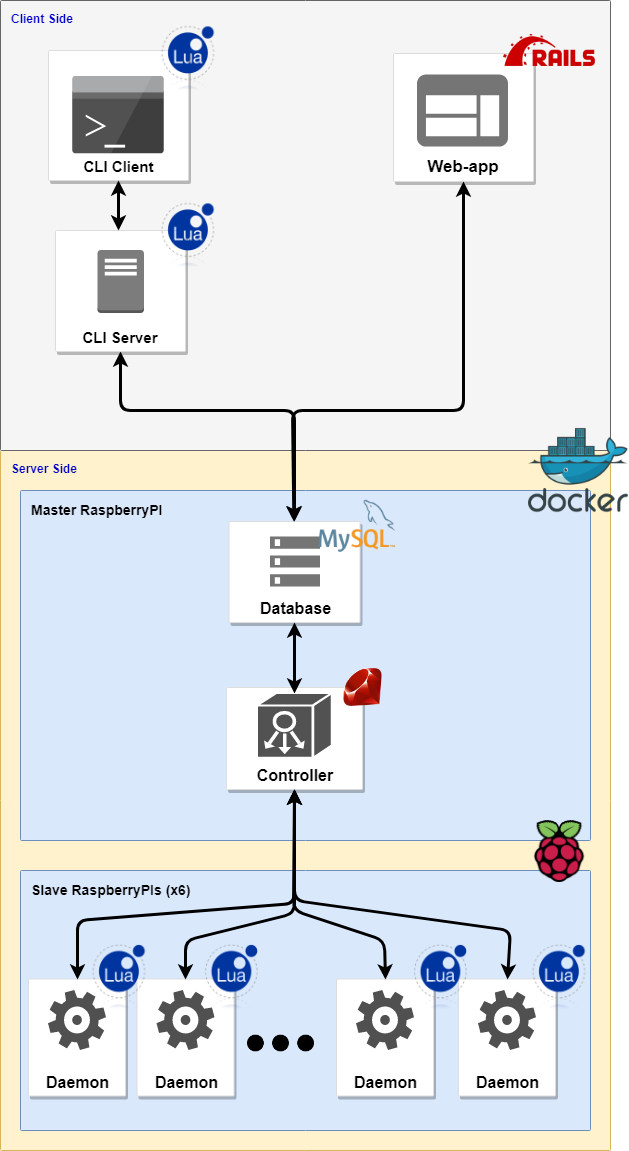
\includegraphics[width=\textwidth]{figures/prev_arch.png}
          \caption{Previous Architecture}
        \end{minipage}
        \hfill
        \begin{minipage}[b]{0.45\textwidth}
          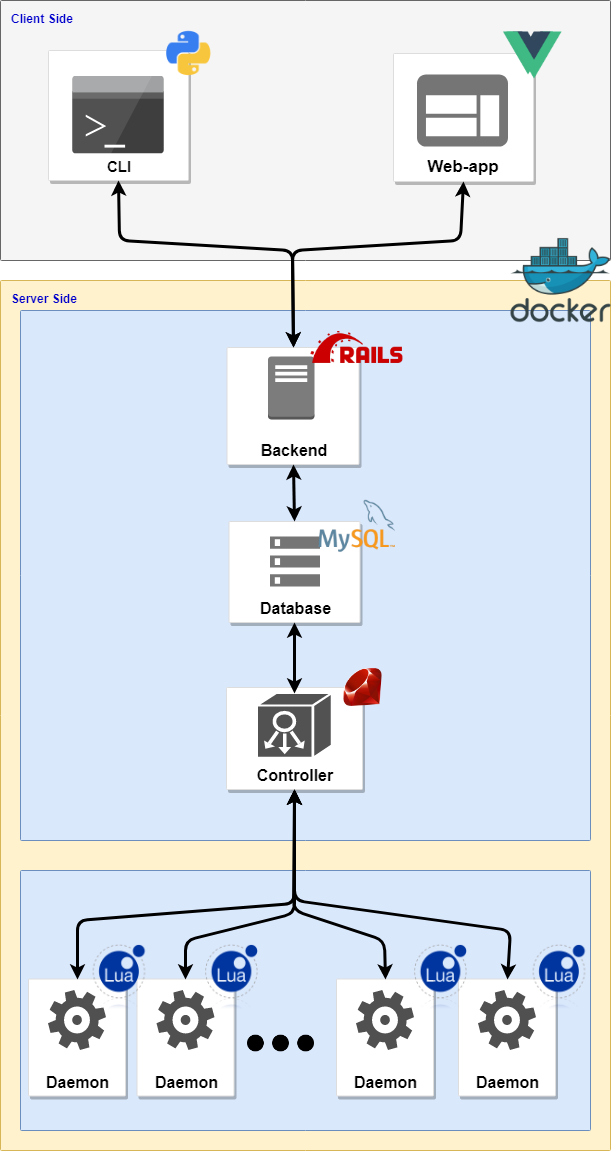
\includegraphics[width=\textwidth]{figures/new_arch.png}
          \caption{Renewed Architecture}
        \end{minipage}
        \caption{Splay Architectural Comparison}
        \label{fig:test}
      \end{figure}

  \chapter{Quality Assurance}

    In this chapter, we will talk about the techniques we used to ensure the
    quality of the project. We put effort in ensuring quality into two
    parts, one being the way we organized ourselves to work together on Splay,
    the other being testing and validation on the codebase.

    \section{Development Methodology}

      Indeed, the fact of being two students on this development project necessarily
      implied a way of organizing ourselves a bit more serious than a
      development project alone.\\

      Thanks to the courses about AGILE methodologies we followed during our
      scholarship, and the both of us having had the occasion of acquiring
      experience in a professional way through internships and part-time jobs,
      we wanted to put to work this knowledge and good practices acquired in
      the project management domain.

        \subsection{Kanban}

          The first tool we put in place, and this from the very beginning of
          the update period of Splay, was a Kanban using the online website
          Trello \cite{trello}. The kanban allowed us to: \\

          \begin{itemize}
            \item Have a clear and precise view about the remaining tasks we had
            to achieve in the backlog, and also about the development state of
            all the other tasks.
            \item Encourage and even oblige ourselves to translate the features
            we had to implement into sufficiently detailed and explicit cards on
            the kanban. This process has the benefit of refining or making
            features the most explicit possible before starting the development.
            \item Have a way of tracking the project's progression and offering
            to all the people related to the project a simple and effective way
            to keep themselves informed about Splay's state.
            \item To focus ourselves on specific tasks and to work in an
            iterative and efficient way.
          \end{itemize}

        \subsection{Testing and Validation}

          The details of our testing and validation suites will be detailed
          in the following section, but we wanted to integrate testing and
          validation processes as part of our development methodology and
          therefore followed a test-driven development approach.\\
          The tests and quality were thus not only a validation technique to
          apply on our work afterward, but a complete part of the development
          and helping us to reach our goals.

        \subsection{Github and Gitflow}

          The project and all the services composing it are versioned using the
          \textit{Git} versioning system and are hosted on the online service
          \textit{Github}.\\
          We therefore organized our work on the Gitflow model. Each feature or
          task we created on the kanban was meant to receive its very own
          branch, starting from the main branch.
          Once the feature finished and tested, a pull request was made asking
          to merge the feature branch with the main branch.\\
          The first benefit of this was obviously to keep the main branch in
          a working state with healthy and finished features. Indeed, as
          we will explain in the following section, we set up a series of tools
          to allow ensuring a branch was passing the tests before allowing any
          merge on master.\\

          \begin{figure}[H]
            \centering
            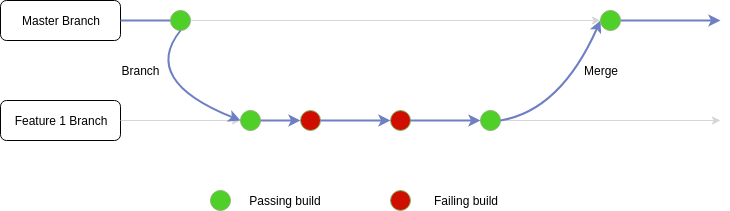
\includegraphics[scale=0.6]{figures/gitflow.png}
            \caption{\label{prev_arch} Gitflow Workflow}
          \end{figure}

          The second benefit of this way of working on the project was to
          permit, once again towards the goal of ensuring quality, code
          reviews. Each time one of us was done with the development of a
          task and was issuing a pull request, the other was assigned as code
          reviewer and was in charge of making this code review, accepting the
          pull request and doing the merge, or to detect errors or bugs as the
          outcome of the code review and therefore to ask for changes to the
          pull request issuer.\\
          Besides the main code review's benefit of reducing the number of
          errors or bugs, this process also allowed each of us to keep itself
          aware and keep itself up to date with all the different changes
          happening on the different services. Indeed, it was impossible for
          us to work together in the meantime on each single service, because
          of the number of services and inter-dependant features we had to
          develop.

    \section{Testing and Validation}

      In this section, we will talk more deeply about the way we wanted to ensure
      the testing and the validation part in the Splay project, whether it be
      at the global system level or at the user functionalities level, each
      section will go through the different services and how we tested it, and
      also how we tested the application globally.\\

      The fact that Splay had no tests at all in the state we receive it
      motivated us into developing a solid test suite for the system.
      Indeed, that fact made our task much harder because we were progressing
      in the dark, each minor change was prone to create dysfunctions that we
      might only notice way later during our work.\\

      The test writing phase took place from the very beginning of our work on
      Splay as part of our development methodology,
      to make sure that we were ensuring the new code's maintainability, but
      also to progressively give Splay's core new tests to have a healthy
      and maintainable final product.

      \subsection{Testing in Web App}

        As we chose Vue as our framework for the web application service,
        all we had to deal with was components. As Vue is organized around
        the use of components, the immediate reward of this was that we would
        be able to write tests dedicated to isolated and simple components.

        \subsubsection{Jest}

          In order to test the components composing the application, we
          went for the Jest \cite{jest} testing framework, which was advised
          as unit testing framework during the project creation.\\

          Testing JavaScript is not always the simplest thing to achieve, the
          ecosystem being in constant evolution with diverse solutions emerging
          trying to fit with the evolution and the apparition of a lot of
          other JavaScript frameworks.\\
          But Jest was a really good pick as testing framework, as it was
          developed by Facebook and designed to fit with the majority of the
          most used front-end framework and this with almost no configuration and
          providing us with a really simple API.\\

          In order to test the application using Jest, we created a directories
          hierarchy reflecting the Vue components hierarchy we created, thus
          a test file corresponding to a component file. In each of these
          test specifications, we decided to target the core part of each
          component: the methods.\\
          Indeed, there is no need to test whether or not a click on a button
          triggers the associated action as this is part of the Vue system. What
          we wanted to test was the triggered action we wrote ourselves and
          were simply functions.\\
          Each file therefore tests that the related components can be
          successfully instantiated among the application, then run a series
          of \textbf{unit tests} validating the methods expected behavior.

        \subsubsection{ESLint}

          Provided almost by default when creating a new Vue project, ESLint
          \cite{eslint} is a JavaScript linter that allows the developer to
          make sure he's not writing code inducing problematic patterns or not
          respecting code guidelines.\\
          This helps to keep a consistent codestyle as we were two people working
          on this project and increase the overall code quality and
          maintainability. We chose not to change any preset of the shipped-in
          ESLint confguration to ensure following common guidelines among the Vue
          community and make sure any developer joining the Splay project will
          be able to work on the web application seamlessly.

      \subsection{Testing in Backend}

        As a reminder, the Backend such as we conceived it has the following
        roles:

        \begin{itemize}
          \item It has the responsibility of handling the database and
          defining its structure.
          \item It must offer a JSON API allowing other applications to interact
          with the system.
        \end{itemize}

        The backend being written in Rails, we therefore have access to the
        ActiveRecord ORM which allows manipulating the database by associating
        tables to models. These models are thus granted with attributes,
        constraints to comply with on these attributes following the constraints
        listed in the database schema, but also granted with methods. This data
        modelization allows us to do model testing.

        The backend role being only to offer a JSON API to the different client
        services through an authentication system using JSON Web tokens, a
        request testing suite should be implemented to validate our set of
        endpoints and the mechanism of authentication.
        The data responses being sent to the calling applications under the form
        of JSON responses, we had to serialize our models and therefore this
        part was also subject to testing.

        \subsubsection{RSpec}

          RSpec \cite{rspec} is a library aiming to ease behavior Driven
          Development on Ruby projects. BDD and TDD (Test-Driven Development) are
          practices we wanted to follow for our work on the Splay development,
          this would allow us to adopt a green-red-refactor work cycles but also
          to focus on writing natural language scenarios and then translating
          them into test scenarios.

        \subsubsection{Model Testing}

          As we made it explicit in upper sections, the Rails ORM layer offers
          a reflexion about the database constraints by representing its
          tables under the form of models granted with attributes, that we can
          enrich with additional attributes, methods and an overlay of
          additional validations (such as validations on attributes
          combinations, or more complex constraints between the models).\\

          This additional abstraction therefore needs to be covered with a
          sufficient validation set, which we did by applying
          \textbf{Model Testing}, challenging that overlay applied to the
          models but also the basic constraints explicited in the database's
          schema.\\

          This testing set is therefore offering a double validation on the
          database field constraints, but also validations on the business
          logic we added in the application.

        \subsubsection{Request Testing}

          The request tests inside the Backend service are the most important
          tests we wrote, in terms of code coverage but also in terms of
          testing the implemented features inside of this Splay service.\\

          The request specs among the RSpec tool are made to simulate
          the behavior of a third-party application sending a request to
          our service and therefore making the whole Rails stack running
          to provide an answer to this request.\\
          Each request is therefore going through those elements:\\

          \begin{figure}[H]
            \centering
            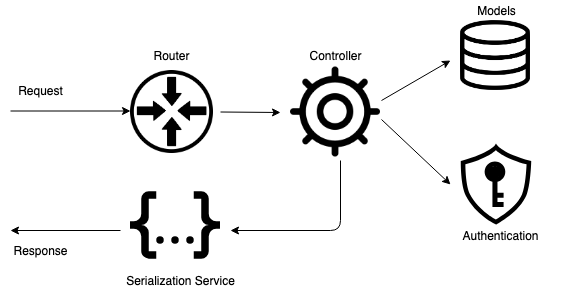
\includegraphics[scale=0.6]{figures/request_test.png}
            \caption{\label{request_test} Request Lifetime in Backend Service}
          \end{figure}

          Each route of the application is tested, exploring different possible
          scenarios for the incoming request (the identification token provided
          is invalid, the token is valid but the requested action is not
          authorized for the associated user). We therefore have a testing set
          that uses the whole application, simply by sending a request and
          making expectations about the awaited response from the application.

        \subsubsection{Code Coverage - Simple Cov}

          We chose to use Simple Cov in combination of the testing applied to
          the Backend. This tool allows to measure the code coverage of Ruby
          application and to provide the developer with useful information
          thanks to its test execution analysis.\\

          Our ambition on the user part of the Splay project was a total recast of
          the services in more simple and maintainable ones, it was therefore
          obvious and simple for us to reach a total coverage of that new codebase
          with a test suite, and thus chose to use that tool.\\

          The benefits we found in using a code coverage tool were the
          following:

          \begin{itemize}
            \item Encourage the TDD approach, as it's easier and better to
            write the tests covering the feature and then writing the feature
            instead of writing the feature and then tests in order to reach
            the coverage level
            \item Ensuring we don't let parts of the code or certain branches
            in conditional statements being untested
            \item Refrain to write useless code. The tests are supposed to cover
            which features should exist, a decrease in the coverage level
            might then spot bad patterns or code being outside the scope
            of the feature.
          \end{itemize}

        \subsubsection{Code Quality - Rubocop}

          We used Rubocop as the last piece of the tool stack designed to ensure
          the code quality within the service. Rubocop is a static code analysis
          tool (linter) allowing to detect violations to a set of rules about
          the code style and good practices (too many lines of code for a method,
          too many variables instantiations, too many conditional branching
          in the code, ...).

      \subsection{Testing in Daemons}

        The Daemon is a critical part of the project as it has to communicate
        with the controller to receive the jobs, run the jobs and return
        information to the controller about the job state. But the Daemon also
        provides the user with a rich Splay library written in Lua.\\
        In the legacy project, only a few tests were present and their
        task was to check the installation and to test some very basic features
        (small functionalities) of the Lua Splay library. Some of those tests
        weren't passing anymore (if they did pass one day), and no testing
        library was used.\\

        We wanted to change this, so we started by adding a testing library
        called Busted \cite{busted}. This library allowed elegant unit testing,
        still under active development and fully integrated with Lua 5.3.\\
        Then we successfully transformed the old existing tests into busted
        tests. With only this single change, we were able to detect some
        anomalies in the lib code and to fix these. We added some test steps
        in the docker image creation to avoid creating malformed images.\\

        Moreover, we added a lot of tests about each modification we made
        (openssl updated, new misc functions, small changes in existing
        functions, ...) and also about the new features.\\
        Sadly the whole Splay lib of the Daemon isn't entirely tested,
        the huge amount of code (some being documented and some not) made it
        really hard for us to make it ourselves during the period of this
        thesis, but still ensuring our work on the Daemon is maintainable
        for future improvement or refactoring.

      \subsection{Integration Testing}

        In order to automatically test the project as a whole, we also wanted to
        develop a functional test suite. This test suite would be relatively
        simple but complete enough to make sure that we could test the developed
        features in a global way among the system, and to achieve this goal we
        just had to translate our user scenarios into test scenarios.\\

        For these functional tests, we didn't use complex technology and
        thought that a Bash scripts series would be more than sufficient to
        reach our goal. Bash scripts could indeed not allow us to recreate user
        behavior using Splay through the web application, but as this
        application is using the exact same API offered by the Backend than the
        CLI application, we could simulate user behavior through that CLI (and
        that's partially the reason why we decided to keep a CLI application
        within the project).\\

        The integration tests were placed in a dedicated directory at the Splay
        project's root, and execute the following actions for each test:

        \begin{itemize}
          \item Cleaning the containers.
          \item Rebuilding the different services listed in the docker-compose
          file.
          \item Starting up the services.
          \item Executing commands through the CLI.
          \item Checking the returned response sent by the CLI and displaying
          whether the test phase has succeeded or failed in the terminal.
        \end{itemize}

        By proceeding this way and with the fact of using our user scenarios to
        determine the actions described in the test suite, we can make sure
        that the implementation of our features is functional and will stay
        functional through the lifetime and evolutions of Splay. Moreover, those
        tests are adding an additional validation layer compared to the tests
        targeting the different services individually. We have here tests that
        are involving each service in concrete scenarios and reflecting real
        working conditions of the project, and also testing interactions
        between the services.

      \subsection{Continuous Integration}

        Once again in a way to ensure quality, the different services were placed
        on the Travis CI \cite{travis} continuous integration platform. Travis
        can be coupled with Github to detect any change on the branches and
        automatically run a test procedure listed in a script and then offer
        feedback on how the test suite went.\\

        Splay being an open source project, that we hope to see growing in the
        future, its collaborative development will inevitably happen through
        the Github organization in which the different repositories are located.\\
        The coupling of Travis with Github allow, in the case of a pull request,
        gather the review about the test execution on the branch asking to be
        merged with the main branch, and therefore to make sure the build is
        clean and the tests are passing before merging the new code, as
        explained before in the Gitflow section.

      \subsection{Overall Testing Suite}

        Here is a figure detailing the whole Splay project with the different
        test suites and procedures that have been described in the previous
        sections so that the reader can get the grasp on the overall
        organization of this.

        \begin{figure}[H]
          \centering
          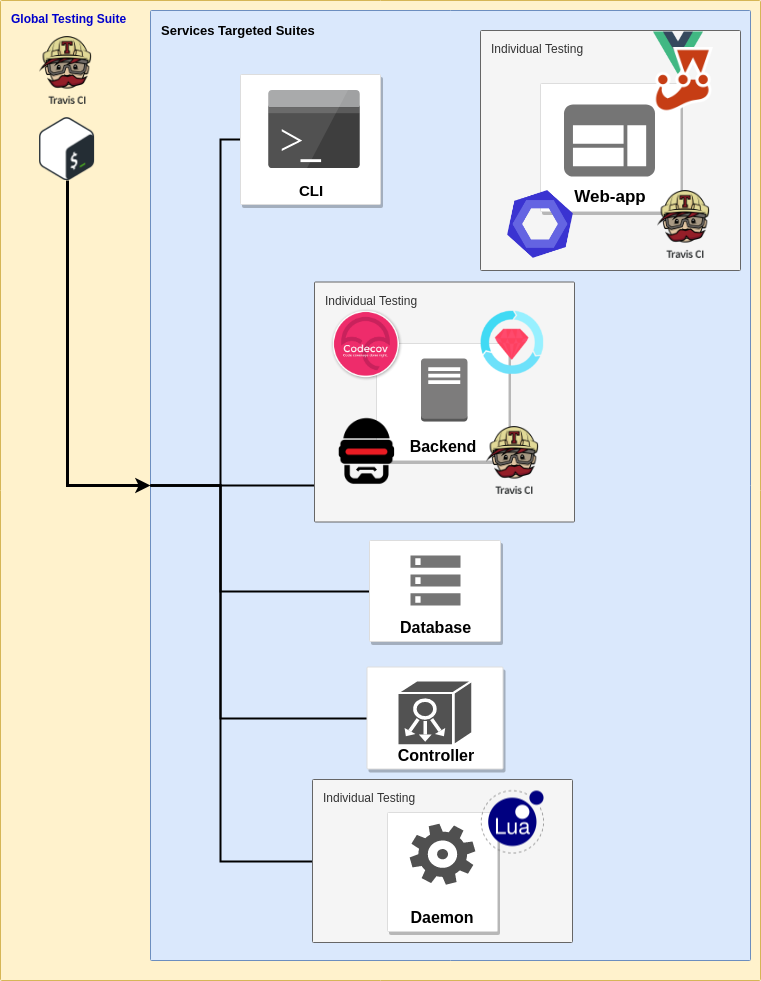
\includegraphics[scale=0.55]{figures/global_testing.png}
          \caption{\label{global_testing} Global Testing in Splay}
        \end{figure}

    \chapter{New Features}

      In the previous chapters, we went through the development of all
      the changes we had to implement in the already existing features
      and the software architecture of the project, and also explained
      in details how we ensured quality insurance among the whole project,
      we now explain the development of the new features we implemented in
      Splay.

      \section{Web Application enhancement}

        The new web application implemented in Vue, which we detailed in
        the previous chapters, has received some of our important new features
        of the project aiming to provide a better user experience: the
        integrated algorithm editor and the topology creation tool.

        \subsection{The Lua editor}

          One of our objectives for the web application was to provide the user
          with a fully integrated Lua editor within the application and
          available during the job creation process.\\
          The idea of entirely building ourselves this editor was quickly
          moved aside, as it would take too much time to achieve and wouldn't
          be a solution allowing easy evolution through time.\\
          We then found a great package named \textbf{Brace}, a browserified
          version of the Ace editor \cite{Ace}. Ace can handle hundreds types
          of different programming languages concerning syntax coloration,
          error handling, line number displaying.\\

          The integration of Ace in the project was really easy and light thanks
          to the available npm package, and the editor now displays Lua code
          perfectly colorized and errors are shown in case of syntax errors.\\

          Sadly, no built-in auto-completion module was available from the
          Brace package. It would have been possible for us to add our own
          auto-complete script in the Ace editor, but that was a too long
          task to achieve for the time we had, we thus decided to move on and
          keep the result as it was.

      \subsection{Topology creation}

        The second objective concerning the web application was to provide the
        user with an easy way to create the topology details he would like
        the job to be run in. The previous and only way to send a topology
        to the server was to write a whole XML file following the ModelNet
        topology representation, a somehow tedious and error-prone process.\\

        The first step in our solution was to create a user interface with
        form fields for each of the components of the topology:

        \begin{itemize}
          \item \textbf{Nodes}: Vvirtual nodes or gateways.
          \item \textbf{Specs}: Set of predefined settings such as the
          bandwith and packet loss rate which would then be used by
          a link.
          \item \textbf{Links}: Linking two nodes, choosing a spec to
          inherit its settings and maybe overriding one of the spec settings
          with its own.
        \end{itemize}

        \begin{figure}[H]
          \centering
          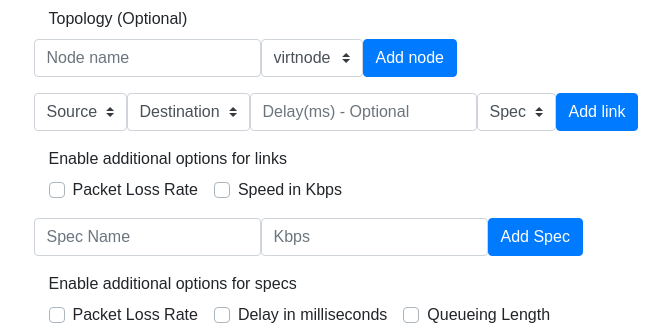
\includegraphics[scale=0.6]{figures/editor_topology.png}
          \caption{\label{editor_topology} UI Topology Editor}
        \end{figure}

        Following this way, we could set validations behind the scenes and
        prevent the user from creating wrong settings such as a link having the
        same node as source and destination and ensure the topology would
        fit in the Splay system. To help the user manage the created
        elements of his topology, a simple summary of his elements is
        output on the page with the related information and a click on those
        allows to delete the corresponding element from the topology.\\
        Indeed, any deletion of a node would delete the link it's associated
        to, or any deletion of a spec would delete the associated links.\\

        \begin{figure}[H]
          \centering
          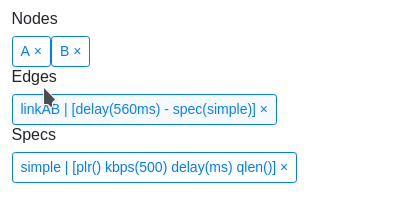
\includegraphics[scale=0.6]{figures/recap_topology.png}
          \caption{\label{recap_topology} Interactive Recap of the topology}
        \end{figure}

        To help the user get a better visualization of his topology, we
        decided to implement a network visualization solution using the
        Cytoscape \textbf{cytoscape} library.\\
        On any update from the form explained above, the change is reflected
        inside our network visualization component adding the new links or
        nodes created by the user so that he can keep track of his topology
        evolution in a more pleasant way.\\

        \begin{figure}[H]
          \centering
          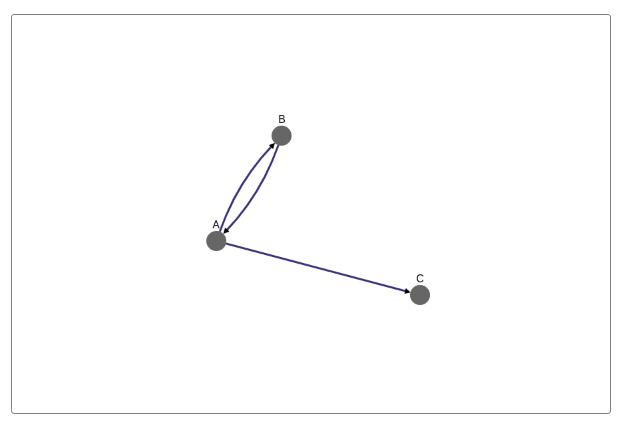
\includegraphics[scale=0.6]{figures/visual_topology.png}
          \caption{\label{visual_topology} visualization of the topology}
        \end{figure}

        Once the user is done editing his topology, he doesn't have to
        do anything more. We created the editor so that the saved entities
        of it (being JSON elements) would be directly transformed into the
        corresponding XML file and sent to the backend alongside his
        job.\\

        However, using a visual tool with buttons and inputs is not always
        the fastest and most practical thing for someone more experienced. We
        thought that some Splay users would probably not want to be obliged
        to play with our topology editor and would keep their topology
        settings in some file alongside with their code.\\
        We therefore wanted to allow the user to play with XML directly
        if he wanted to, offering the following service:

        \begin{itemize}
          \item A user creating the topology could also translate what's
          displayed in the visual editor into the XML definition.
          \item A user creating the topology could directly paste
          his XML topology in some editor and also have the option of
          translating it into our visualization solution.
        \end{itemize}

        Addressing these two issues was an extremely easy task, the job of
        converting the topology in XML was already available and done on
        the job submission. We therefore reused the Brace package used
        for the Lua code editor to create an XML Topology editor.\\
        The user could then trigger an XML creation into the Brace editor
        before sending the job, or paste its code into the Brace editor and
        then ask for reflecting the XML topology into the visual editor. It
        was just then the matter of parsing the XML and generating the
        corresponding JSON entities, reusing the functions we already wrote
        for the Vue components composing this global feature.

        \begin{figure}[H]
          \centering
          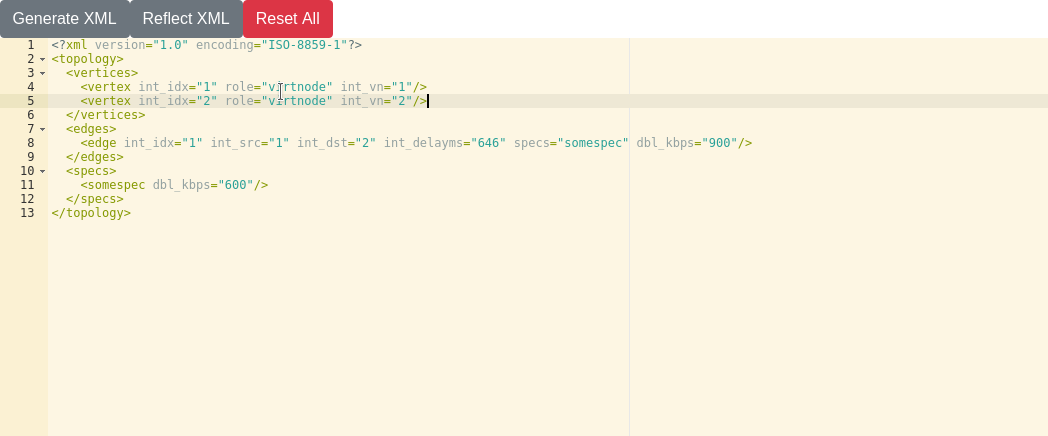
\includegraphics[scale=0.5]{figures/xml_topology.png}
          \caption{\label{xml_topology} XML Display and Editor}
        \end{figure}

    \section{Fault injection}

      The fault injection feature (or crash point) is achieved on the daemon
      side of the application. Indeed, we wanted to be able to trigger a crash
      of the code in the middle of the execution tree, therefore only the
      daemon was able to handle with precision the crash.\\

      We therefore made the decision to use a domain specific language (DSL)
      for the crash management so that a user could define the crash point
      in the Lua code as a comment. During the job execution phase, just before
      executing the user code, we parse the code and gather those crash
      points to manage the crashes.

      \subsection{Domain Specific Language (DSL)}

        We defined our small domain specific language to be simple to use
        for the user and flexible enough for the parsing phase. This DSL
        needed to be integrated into the Lua code without forcing the user to
        modify its algorithm code and trying to avoid totally crashing
        the daemon in case of the crash points specified by the user were
        not correct.\\
        Also, the difference in terms of th number of lines of code between the
        source code before and after the parsing needed to be the same in
        order to keep the feedback error messages right (getting the same line
        number when locating the error).\\

        For these reasons, we designed the feature so that a crash point has
        to be represented as \textbf{one line} of code and beginning by
        two hyphens (--) which indicates a Lua comment.\\
        To avoid interpreting any other comment, those crash points must
        contain the keyword \textit{CRASH POINT}. Achieving this by comments
        was probably the best option, so that the real code doesn't get any
        interference with our crash point functionality. The crash then
        happens exactly where the crash point is defined, it is therefore
        possible to make the execution code crashing anywhere (thread, middle
        of a function, etc...)\\

        Secondly, a fault is defined by a type, the moment it should occur and
        on which node it should occur. These characteristics also needed to
        be specified within our DSL. Each characteristic follows the
        \textit{CRASH POINT} keyword and are separated by a colon, and are
        defined by their keyword and values if needed.

        \begin{itemize}
          \item First, the chosen nodes to be affected by the crash must be
          specified. For this purpose, the user must add the ids of the
          affected nodes separated by a space (ids begin at 1 -> number of
          daemon used).
          \item The type of crash can be specified by its name and optional
          parameters
          \item The moment where the crash occurs
        \end{itemize}

        Our final DSL looks like this:

        \begin{lstlisting}[style=MyBash]
-- CRASH POINT id_splayd [id_splayd [...]]: <TYPE>: <WHEN>
<TYPE> => STOP | RECOVERY <float>
<WHEN> => AFTER <int> | RANDOM <float>
        \end{lstlisting}

        As the reader can see, we defined two types of crash and two ways to
        define the moment of the crash.\\
        A stop crash means that the node will die forever. Cconversely, a
        recovery crash means that the node will crash and recover after a
        number of seconds specified by the user (float number).\\
        Concerning the moment of the crash:

        \begin{itemize}
          \item The \textbf{AFTER} keyword means that the user specifies the
          number of loops to achieve before the crash occurs. For example,
          the value 5 in a beginning of the loop means that this loop will
          execute 5 times before triggering the crash, whereas 0 triggers
          an immediate crash.
          \item The \textbf{RANDOM} keyword means that the user specifies a
          probability between 0 and 1 that the node crashes each time it
          encounters the crash point through the code execution. For example,
          if the user specified 1, the crash will occur at first execution
          (similar to AFTER 0).
        \end{itemize}

        Here are some positive examples of crash points using our DSL:

        \begin{lstlisting}[style=MyLua]
-- Crash forever the node 1 and 2 at the 4th passage
-- in the code
-- CRASH POINT 1 2: STOP: AFTER    3

-- At each time that the code (node 1) pass by this comment,
-- there is 0.0002 chance to crash the node 1
--CRASH POINT 1: STOP: RANDOM 0.0002

-- Crash immediately when the comment is encouter in
-- the node 1, but this node will recover after 2 sec
-- CRASH POINT 1: RECOVERY 2: AFTER 0

-- Have one chance on two to crash at each pass for
-- the node 1, 2, 3, 4, 5. But recover immediately
-- CRASH POINT 1 2 3 4 5:RECOVERY 0:RANDOM 0.5
          \end{lstlisting}

        We also added some negative examples (won't trigger any crash
        and won't crash the daemon):

        \begin{lstlisting}[style=MyLua]
-- Won't work because Crash point not in uppercase
--Crash Point 1 2: STOP: AFTER 3

-- Won't work because no node is specified.
-- CRASH POINT:RECOVERY  965:   AFTER 3

-- Won't work because RECOVER is not a valid
-- type (but warning expected).
-- CRASH POINT 1 2:RECOVER 1: AFTER 3

-- Won't work because TIME is not a valid type
-- for now (but error expected).
-- CRASH POINT 1 2:RECOVERY 1: TIME 3
        \end{lstlisting}

      \subsection{Parsing}

        The code parsing phase is achieved just before that the user code
        is effectively launched on each node (daemon). The parsing will
        create a table with information about each crash point found in the
        user code and which nodes this crash should occur on.\\
        This table is then saved in a library called \textit{"splay.crash"},
        and is used by the nodes to get the crash information using an id
        number which will retrieve the corresponding crash information.\\

        The parsing phase actually assigns to the nodes a new code where the
        crash points comments specified by the user are transformed and
        replaced (if no error is found) by a function call containing the
        crash id number. Therefore, when the code executes, the crash
        function will access the library and will act depending on what
        information is stored into the crash table (type of crash,
        moment of trigger).

        The parsing handles any error the user could have done about the
        syntax of the crash point.\\
        Parsing is done line by line and if any error is found (also error
        about the parsing code itself), the concerned line will be unchanged, and
        a warning or error message will be written in the logs.\\
        This feature is fully written in Lua using the basic regex matcher of Lua
        \cite{RegexLua} (it isn't a complete Regex implementation).

      \subsection{Execution}

        We saw how exactly we defined our DSL and how we achieve the parsing,
        we shall now see in detail how the crashes exactly happen, how they
        are handled and how the nodes recover if they have to.\\

        The main problem with the Lua language is that the multithreading
        is non-preemptive, this means that we cannot stop a thread from the
        outside \cite{CoroutineLua}. The only way to stop directly the Lua
        interpreter and kill any other thread is to exit the program using
        an OS function (os.exit). We also have the possibility of sending an exit
        status code to the process, which is very convenient for knowing
        if we need to restart or stay down after a crash point was
        triggered.\\

        With this way of exiting, we can create artificial crash points which
        will immediately kill every coroutine (threads) of Lua and its
        current execution. Moreover, we can pass special exit status codes
        in order to send messages to the parent process.\\
        In order to use these exit codes, we created a fork (available from
        the C splay library) before parsing the crash point and executing
        the user code.\\
        Therefore, the child process will execute the parsing of the crash
        point and proceed to the code execution, and the parent process will
        wait to receive the exit status code of its child. We added a Lua
        function (waitpid) for this purpose and used the original waitpid
        of C \cite{waitpid}.\\

        When the child process terminates (either in a normal way or because
        of a crash), the parent process checks the exit status code and act
        accordingly. If the exit status code is 65 or 66, it means that a
        crash has been triggered (or that the user wants to exit
        with one of these values).

        \begin{itemize}
          \item \textbf{65}: Means a STOP crash, no restart is needed
          \item \textbf{66}: Means a RECOVERY crash
        \end{itemize}

        The recovery crash is then achieved recursively, the parent process
        creating another fork, and the crash table is reset when reparsing
        the original code. Moreover, when it is a recovery crash, the user
        can define the downtime. Our simple solution to achieve this is by
        using the non-preemptive feature of Lua and forcing the process
        to sleep x seconds without any yield coroutine (therefore other
        coroutines can't execute any code) before crashing.

  \chapter{Use Case}

    We will take the example of a student following a course on distributed
    applications and distributed systems who wants to prototype the Raft
    leader election algorithm on five different nodes. He chose to use
    Splay for his tests using his own laptop (or if available, a cluster
    of mini-computers) and right now he has no available installation of the
    Splay system. We are going to describe the different steps that our
    student will go through by using the Splay application.\\

    First, he needs to install a Splay environment on his own computer. Then,
    with the help of the Splay library, he will build a basic Raft leader
    election implementation.\\
    Following this, he would like to understand what's happening during the
    execution of Raft by showing an animation of the evolution of the
    endpoints states.\\
    Moreover, he would like to test its algorithm implementation through
    different network topologies and theRafter analyse its solution's
    robustness by adding fault injection in key parts of the algorithm.\\
    To conclude, one of his friends sent him a slightly different version
    of the algorithm avoiding some writings on disk, and he would like to
    prove by example that his friend's solution isn't valid.

    \section{Installation of Splay}

      The student only has his laptop to work on his distributed algorithms
      courses, and hopefully, he found out on the Splay's main Github
      repository \cite{SplayV2Git} that the installation doesn't depend on
      any operating system or hardware. The README file of the Github project
      precisely describes how to install Splay. Then, following the
      instructions, he clones the main repository and installs docker and
      docker-compose on his computer.\\
      In order to run Splay on production mode, he runs the following
      commands in his terminal emulator: \\

      \begin{lstlisting}[style=MyBash]
docker-compose -f docker-compose.prod.yml up -d web_app controller
# 7 daemons because it is recommended to have more than needed
docker-compose -f docker-compose.prod.yml up -d --scale daemon=7
      \end{lstlisting}

      The images are downloaded from prebuilt images (from dockerhub) for
      each service, some little wait time is requested for this download
      phase and for each service to start.\\
      Once this is done, the student has access to the web application of
      the Splay system, using his favorite web browser with this url:
      \url{http://localhost:8080/}.\\
      He creates his own account by registering on the platform, opens a new
      session (which will be kept open for the next time he wants to use
      the system) and now he can easily prototype his own distributed job.

    \section{Implementation of Raft in Lua}

      After the successful easy installation, the real work can start, our
      student will create his own implementation of Raft using the Splay
      library.\\

      \textit{Raft is not a trivial algorithm, but still an easily understandable
      one. The algorithm we will present in the next subsection is based on
      some papers \cite{RaftPaper} and articles/courses \cite{RaftSlide}
      \cite{RaftSite}. We have done the Lua code of the Raft consensus leader
      election part with the help of the Splay lib \cite{SplayLib}.
      We will therefore present and focus only on the election subproblem of
      Raft because the log replication heavily increases the complexity and
      the readability.}

      \subsection{Creation of the Algorithm}

        The student finally created the Lua version of the Raft leader
        election subproblem, which is not trivial, but made really
        understandable through comments in the code:

        \lstinputlisting[style=MySmallLua]{raft_election.lua}

      \subsection{First Results}

        After having wrote the Raft's code, he wants to try it on five nodes
        and without any network topology (that means all nodes are directly
        paired to each other without any latency).\\
        Once he sent the job, it can be observed in the logs that a node
        effectively becomes the leader and it is sending heartbeats to avoid
        an election process from the other nodes:

        \begin{lstlisting}[style=MyBash]
2019-05-30 08:20:10.0501 (3)  2: Election Trigger -> term+1, become candidate
2019-05-30 08:20:10.0504 (3)  2: Send vote request to node 1
2019-05-30 08:20:10.0506 (3)  2: Send vote request to node 3
2019-05-30 08:20:10.0508 (3)  2: Send vote request to node 4
2019-05-30 08:20:10.0508 (3)  2: Send vote request to node 5
2019-05-30 08:20:10.0522 (2)  3: RPC Request Vote FROM 2.0 Term: 1.0
2019-05-30 08:20:10.0527 (2)  3: Stepdown: 1.0 > 0
2019-05-30 08:20:10.0525 (4)  5: RPC Request Vote FROM 2.0 Term: 1.0
2019-05-30 08:20:10.0525 (4)  5: Stepdown: 1.0 > 0
2019-05-30 08:20:10.0539 (1)  4: RPC Request Vote FROM 2.0 Term: 1.0
2019-05-30 08:20:10.0539 (1)  4: Stepdown: 1.0 > 0
2019-05-30 08:20:10.0557 (7)  1: RPC Request Vote FROM 2.0 Term: 1.0
2019-05-30 08:20:10.0557 (7)  1: Stepdown: 1.0 > 0
2019-05-30 08:20:10.0576 (3)  2: Vote Request result 1.0: true from 3
2019-05-30 08:20:10.0576 (3)  2: Vote Request result 1.0: true from 4
2019-05-30 08:20:10.0576 (3)  2: I Become the LEADER !
2019-05-30 08:20:10.0580 (3)  2: Vote Request result 1.0: true from 5
2019-05-30 08:20:10.0583 (3)  2: Send append entry (null) to node 1
2019-05-30 08:20:10.0585 (3)  2: Send append entry (null) to node 3
2019-05-30 08:20:10.0587 (3)  2: Send append entry (null) to node 4
2019-05-30 08:20:10.0587 (3)  2: Send append entry (null) to node 5
2019-05-30 08:20:10.0599 (3)  2: Vote Request result 1.0: true from 1
2019-05-30 08:20:10.0608 (4)  5: RPC Append entry FROM 2.0 Term: 1.0 Entry: null
2019-05-30 08:20:10.0611 (1)  4: RPC Append entry FROM 2.0 Term: 1.0 Entry: null
2019-05-30 08:20:10.0617 (7)  1: RPC Append entry FROM 2.0 Term: 1.0 Entry: null
2019-05-30 08:20:10.0622 (2)  3: RPC Append entry FROM 2.0 Term: 1.0 Entry: null
        \end{lstlisting}

    \section{Timeline Animation}

      Before testing the robustness of his solution, our student wants to
      see how the network and the connection is evolving during his job's
      execution.\\
      For this purpose, Splay contains a small tool designed to parse the
      logs and allow the user to see that evolution during the job's
      execution. This tool is embedded in the web application with some
      JavaScript and shows the node states (follower, candidate or leader),
      shows if a packet is travelling between two nodes and shows time
      indications following the animation. This tool uses the vis.js library
      \cite{VisJS} (dynamic graph library) and the Raft code has been slightly
      modified in order to print the appropriate logs (code can be found here
      \footnote{\url{https://github.com/splay-project-v2/cli/blob/master/app_test/raft_election_anim.lua}}).\\

      This tool takes a text-based log, a speed factor and auto-connect
      checkbox as inputs, and here, is used to illustrate our Raft election
      process evolution over time. We reprensents, on the graph, the node (job) state
      by different color : blue for follower, green for candidates and red for the leader.
      Also, network packets currently travelling between nodes, change the color
      of the directed edge into black and become larger (depending of number of packets).

      \begin{figure}[H]
        \centering
        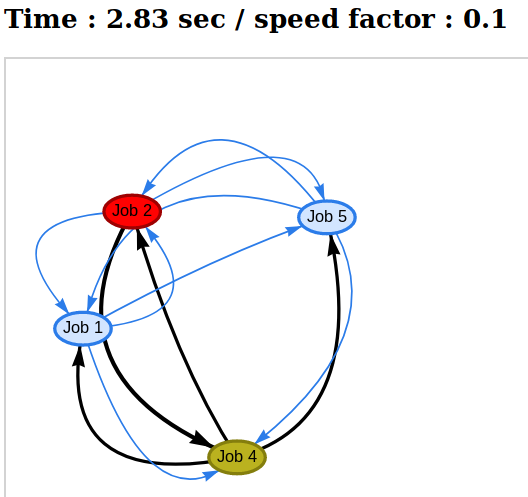
\includegraphics[width=0.7\linewidth]{figures/user_case/anim_pres.png}
        \caption{Timeline animation example}
      \end{figure}

      If we observe the leader election from the first result (without
      topology network and no crashes) with this tool, we won't see clearly
      the evolution of the nodes states, because the leader election finishes
      very quickly (< 8 ms) and it is hard to capture the visualisation of it
      (or with an extreme small speed factor).\\
      The main reason is the lack of latency between nodes. Indeed, without
      topology the RPC messages travel instantaneously, and then a candidate
      get its vote granted really fast (and thus becomes the leader directly,
      with almost no chances of conflict with another node).

    \section{Robustness of solution}

      The student is not totally sure that his solution is correct, and he would
      like to try to break his Raft election by testing it with different
      network settings and by adding some fault injection in the critical
      parts of the process.

      \subsection{Topology settings}

        After testing the algorithm in a perfect network environment
        simulation, the student tries it with three different network
        topology configurations created through the network topology tool on
        the web application.\\
        Here are representations of the topology, with specifications on
        the edges between nodes-routers and routers-routers.\\
        These specifications are focused on latency only, bandwidth constraints
        are not really influencing Raft as it is producing small and few
        packets.

        \begin{figure}[H]
          \centering
          \begin{subfigure}{0.6\textwidth}
            \centering
            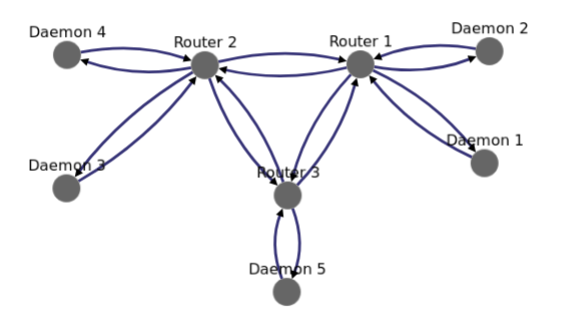
\includegraphics[width=1.0\linewidth]{figures/user_case/raft_topo_1.png}
            \caption{First topology - Normal: Router-Router -> 5 ms of delay and 10000kbps, Daemon-Router -> 15 ms od delay and 1500kbps}
            \label{fig:topo1}
          \end{subfigure}
          \centering
          \begin{subfigure}{0.6\textwidth}
            \centering
            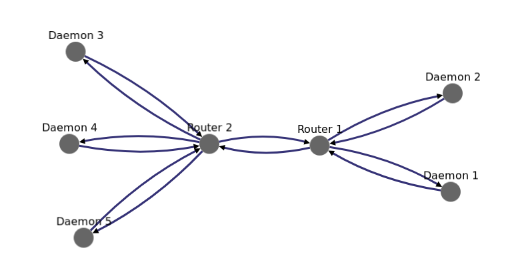
\includegraphics[width=1.0\linewidth]{figures/user_case/raft_topo_2.png}
            \caption{Second topology - Two sites: Router-Router -> 150 ms of delay and 15000kbps, Daemon-Router -> 10 ms od delay and 15000kbps}
            \label{fig:topo2}
          \end{subfigure}
          \centering
          \begin{subfigure}{0.6\textwidth}
            \centering
            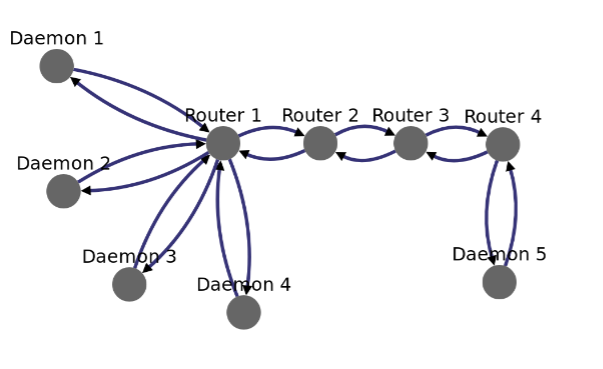
\includegraphics[width=1.0\linewidth]{figures/user_case/raft_topo_3.png}
            \caption{Third topology - Extreme: Router-Router -> 200 ms of delay and 15000kbps, Daemon-Router -> 15 ms od delay and 1000kbps}
            \label{fig:topo3}
          \end{subfigure}
          \caption{plots of three topologies}
          \label{fig:topologies}
        \end{figure}

        The student then tries his implementation of the three configurations,
        the log results show that Daemons succeeded at achieving the leader
        election and quickly stabilize (one becomes the leader, the other
        become followers) in those different network configurations.\\
        But as we know, Raft election is also fault-tolerant when a majority of
        nodes are still actives, the user therefore would like to test this
        fault-tolerance characteristic of the algorithm.

      \subsection{Fault injection}

        The user now wants to test the correctness of his implementation
        essentially by making the leader crash, but also the other nodes.\\
        When the leader crashes, the student expect from the Raft specification
        that an other leader election will be triggered by the remaining
        nodes, and therefore a new leader will be elected.\\
        To achieve this, the student adds a recovery crash point where the
        heartbeat is triggered in the code:

        \begin{lstlisting}[style=MyLua]
...
function heartbeat()
-- CRASH POINT 1 2 3 4 5: RECOVERY 0.5: AFTER 5
for i, n in pairs(job.nodes) do
...
        \end{lstlisting}

        This crash point will only be triggered by the leader (as heartbeat
        is only used by the currently elected leader) after five heartbeats
        (when the 6th is called).\\
        When the crash happens, the node will recover after 0.5 seconds.\\
        Also, the student adds other crash points not depending on the
        node's state but triggering less often. For example, when a RCP vote
        request is received:

        \begin{lstlisting}[style=MyLua]
...
function request_vote(term, candidate_id)
  -- CRASH POINT 1 2 3 4 5: RECOVERY 0.5: RANDOM 0.05
  print("RPC Request Vote FROM "..candidate_id.." Term: "..term)
...
        \end{lstlisting}

        This one will be triggered by a node when it receives a vote request
        from a candidate with a probability of 0.05 (one chance on 20).\\
        The student creates other crash points in another key step of
        the algorithm (when a vote is granted) to observe the behavior of
        the Raft election when there is a fault.\\

        After some test, he checks the logs for the different topology
        settings, and he sees that everything went as expected. Indeed, when
        the leader crashes, another node will trigger a new leader
        election and become a candidate. If there is no conflict with another
        candidate (election triggered by two nodes at the same time), this
        candidate will become leader and only one node can be the leader
        at the same time.

      \subsection{Animation results}

        Now the student have tried his Raft election implementation on
        different topologies and with some crash points, he can observe some
        interesting results thanks to the animation tool.\\
        A complete Raft election can be divied in multiple steps. The next
        figure shows a complete election process with a conflict between
        three candidates (candidates asking almost at the same time vote
        requests to the others).\\
        In this case, nobody gets the majority of vote, therefore another
        election will be triggered with a bigger term at some point.
        And with this new election, the candidate who received enough votes
        will become the leader (no conflit this time).\\
        Note that conflicts happen rarely with 3 candidates, because the
        leader timeout is well balanced thanks to randomization and the
        topology used is not an extreme case (topology 2 \ref{fig:topo2}).

        % Show four step of election: all followers -> two candidate -> one leader -> leader + heartbeat
        \begin{figure}[H]
          \begin{subfigure}{.45\textwidth}
            \centering
            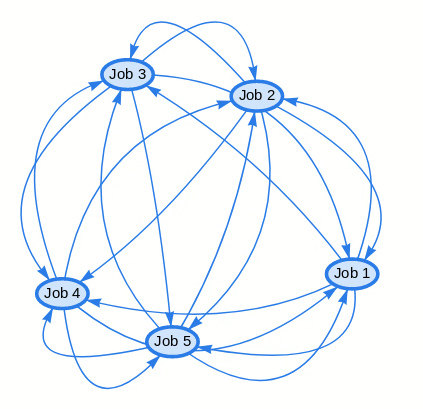
\includegraphics[width=1.0\linewidth]{figures/user_case/election_1.png}
            \caption{When all nodes are awaken and they are all followers (begin state)}
            \label{fig:ele1}
          \end{subfigure}\hspace{0.1\textwidth}
          \begin{subfigure}{.45\textwidth}
            \centering
            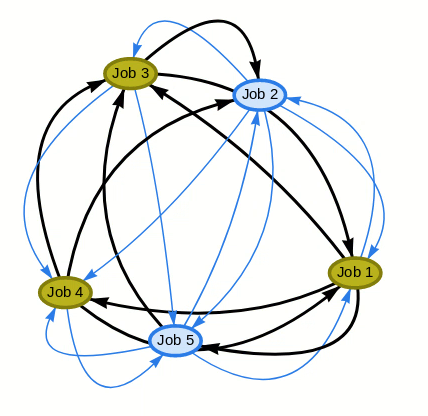
\includegraphics[width=1.0\linewidth]{figures/user_case/election_2.png}
            \caption{Three candidates for the leader job -> conflict, none become the leader, the majority is sliped}
            \label{fig:ele2}
          \end{subfigure}
          \begin{subfigure}{.45\textwidth}
            \centering
            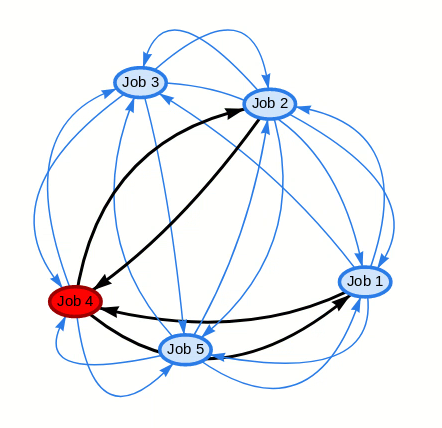
\includegraphics[width=1.0\linewidth]{figures/user_case/election_3.png}
            \caption{New leader election from job 4 with a bigger term -> becomes the leader when receives the majority}
            \label{fig:ele3}
          \end{subfigure}\hspace{0.1\textwidth}
          \begin{subfigure}{.45\textwidth}
            \centering
            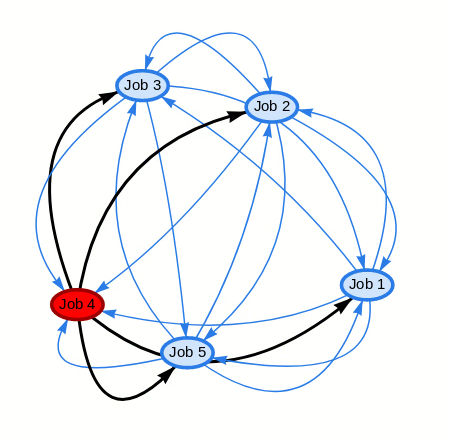
\includegraphics[width=1.0\linewidth]{figures/user_case/election_4.png}
            \caption{The leader (job 4) sending heartbeat to other nodes to avoid a new leader election}
            \label{fig:ele4}
          \end{subfigure}

          \caption{Raft election animation from the parsing of a job's log, with the topology in figure \ref{fig:topo2}
          and crash points for the leader}
          \label{fig:election}
        \end{figure}

        In this case no node crashes but we can show that even when a crash
        happens, Raft is fault-tolerant as long as there is a majority of
        nodes alive (3 in this case). If there is only one or two nodes alive,
        the election can't be achieved until a third node wakes up.\\
        The animation shows that, when the leader crashed, one or multiple
        nodes triggered a new leader election process.\\
        Crashes can also happen on a follower or candidate node, which won't
        disturb the raft process as long as there is a majority of nodes
        running.

    % \section{Buggy code proof}

      %A friend of the student (Goerge) sent him a supposedly better code, but he is not
      %convinced. Indeed, Goerge assume that we the vote (voted\_for) don't need to be saved
      %in the persistant state. For him, it is downgrade the performance and the
      %code is still correct. A version of the code can be find here TODO

      %The student has, however some doubts about this "upgrade", and then he decides to find a specific case
      %where the Raft election fails to choose only one leader. \\
      %After some search, he finds a way to create a example where two leader running in same time with the
      %helped of crash point at certain points

      % Show buged piece + fault injection -> buggy log

  \chapter{Conclusion}

    We'll first conclude this report by going through a list of improvements
    idea over the project, and then summarize our global achievements on the
    project comparing our initial objectives with the work we achieved.

    \section{Improvements}

      This section will hold our thoughts about the further improvements
      that could be made on the project, these improvements are mainly about
      our new features, the improvements that could be made on the "legacy"
      services and also some improvements thoughts about the security.

      \subsection{New features improvements}

        Our new features on the Splay system may be improved over the future
        and we will expose our ideas and thoughts for each one of these
        features.

        \subsubsection{Lua editor}

        During the development of our features, we noticed that the Lua Editor
        is probably the less important one. The main reason making this feature
        the less important is that most of the time, users create their own Lua
        scripts on their favorite editor and then apply a copy-paste on the
        system.\\
        A fully integrated IDE with a Lua an installed Lua package offers more
        than our editor, but with little improvements, our editor could equal
        any other:

        \begin{itemize}
          \item \textbf{Basic Auto-Completion}: A basic auto-completion can be
          done for keywords (as any other IDE) and for named functions with
          the help of the Ace Editor package.
          \item \textbf{Specific Auto-Completion}: The integration of the Splay
          Lua library to the auto-completion feature with some hints would
          be a great achievement and make the Lua editor an even better
          option than an IDE.
          \item \textbf{Color Theme}: Ace allows to set a color scheme for
          the editor, an option for the user to change this color scheme
          might be a great option to make the development environment
          truly enjoyable.
        \end{itemize}

        As Ace can handle a lot of different languages, if in any further
        improvement a decision to switch the daemon technology was made (see
        next section about refactors), then it would be easy to change the
        targeted language.

        \subsubsection{Crash point}

          The crash point feature now handles two types of crashes and two
          behavior to adopt in case of a crash. This feature is very useful
          to simulate a hard stop of a machine (power loss, for example).\\
          However, we could improve this by adding new types of crashes like a
          network crash or network compartmentalization meaning that the
          nodes would still be running but could not communicate anymore
          with other nodes during the downtime.\\
          For this purpose, we could modify the socket wrapping done to achieve
          topology (or creating a new one) where our crash library could ask
          for restrictions over the network simulation.\\

          Moreover, we can imagine providing the user with more control options
          to configure more precisely what should happen in case of crash or
          when the crash should happen. For example, crashing when some
          precise conditions are met.

        \subsubsection{Topology Creation}

          The actual topology creation through the modern interface is very
          useful to build a precise topology in a quick way. However, we have
          a non-exhaustive list of ideas that could improve this feature, but
          wasn't achievable now because of time constraints:

          \begin{itemize}
            \item \textbf{Modifications of items on click}: For now, it is hard
            to modify existing edges, nodes or specs. The user needs to remove
            the specified item or modify it in the XML code, therefore
            an option to modify existing items through a form would be a good
            idea.
            \item \textbf{Edge in both directions}: Right now, the user can only
            add directed edges between nodes, adding an option to directly
            created edges in both directions would be a good idea and
            avoid double work with the directed edges through the form.
          \end{itemize}

      \subsection{Refactor of old services}

        We have rebuilt some parts of Splay using modern technologies as
        explained in the related section, but we haven't made a complete
        refactor of the daemon and the controller. We think that those two
        services would need, in the future, a complete refactor or even be
        rewrote maybe using newer technologies. A database schema cleaning
        would also follow, as some fields of the various entities may no be
        useful anymore.

        \subsubsection{Daemon}

          The daemon is, with the controller, one of the most critical parts of
          the project and has been built using Lua \cite{Lua}.\\
          During our work, after having stabilized the project, we encountered
          a lot of unused code lines, small bugs and code repetition in the
          Daemon codebase and we therefore carefully fixed those issues when
          encountered.\\
          We therefore reduced the usage of the Splay library by the Daemon
          and ended up with a lot of unused and undocumented code in this
          library. For these reasons, we think that a complete check of the
          Splay Lua library should be performed (with the help of a previous
          maintainer of the project) to provide it with helpful documentation
          that would ease its usage and would allow enhancing our busted test
          suite.\\

          Moreover, we saw by the end of the project that the socket
          topology restriction wasn't actually taking into account
          the packet loss rate and the queue length (maybe this feature was
          a work in progress in the latest version of the legacy codebase).\\
          Therefore, the topology settings that can be tweaked are limited to
          the bandwidth and latency.\\
          Furthermore, we saw that the topology restriction is based on the
          \textbf{IP} combined to a single port number, this causes unknown
          client sockets (because the port is different than the server port)
          and useless restrictions. For all these reasons, the socket topology
          (coming with the SplayNet module) needs to be improved.\\

          A radical solution to clean this service and offer a new alternative
          to users would be to completely rewrite the Daemon service using
          another technology.\\
          The best alternative for the language would be Python, Python being a
          very popular language with a supportive community and constantly
          updated, having rich libraries offering complete sets of tools.\\
          However, the main problem of this solution would be the performance
          offered by vanilla Python compared to the very small core of Lua and
          its C integration. But the main drawback of Lua is evolution, Lua has
          not received major updates since 2014 and the libraries used in this
          project are not evolving too. Moreover, the tiny core of Lua forces
          the user to write its own basic functions that are built-in in many
          other languages and thus were placed in the Splay lib in our case.\\
          This results in a greater number of lines of codes for the Splay lib,
          which thus includes more chances of bugs.\\
          Going back to the performance question, using a just-in-time compiler
          such as PyPy \cite{PyPy} to significantly boost the performance and
          using some distributed libraries to quickly create a new Splay library
          may be a solution.

        \subsubsection{Controller}

          The controller service is the brain of the project, it manages the
          different daemons, reads new data from the database and writes the
          results, dispatches the different jobs.\\
          Despite being such a central piece of the project, the code is still
          badly documented and still needs an advanced cleanup in its
          different parts, and it is also poorly tested even after we worked
          on it. We may therefore propose two different ways to increase
          the quality and maintainability of the controller for future
          development phases:

          \begin{itemize}
            \item Using full object-oriented with sequel \cite{Sequel} model
            object for each table of the database. The SQL queries are now
            raw ones which can be insecure (in case one forgets to manually
            check against injections) and which is hard to read.\\
            A sequel model object allows every operation on a SQL database
            through function calls in a nice a concise Ruby way, avoiding
            SQL error syntax and most importantly it is independent of the
            database management system.
            \item A meticulous refactor of some part of the controller may be
            a good idea, and more specifically the management of jobs sent to
            the daemons (a Ruby class named Jobd and its children classes), we
            indeed found most of the controller bugs in this part.
          \end{itemize}

      \subsection{Security Aspects}

        In the description of the legacy project, we saw that the user's job is
        supposed to be running in a restricted area and the project is secure in
        general.\\
        But with further analysis, we found out that the project wasn't secure
        in various ways:\\
        \begin{itemize}
          \item The restriction on the socket can actually be completely
          bypassed. Indeed, using Lua there is a way to unload a package
          dynamically (package.loaded["name\_package"] = nil). Using this
          technique, we can unload the socket package (that was loaded with a
          restriction) and reload it with the corresponding statements placed
          at the beginning of the job code and the restriction won't exist
          anymore.
          \item SQL calls in the controller are using string interpolation,
          in most of the cases, the call is secure manually adding escape
          characters in the string. Indeed, there is no security issue if
          each call is protected with escaping, but the fact this is done
          manually is a bad practice and will create a security issue if
          any verification is mistakenly skipped by a developer.
        \end{itemize}

        We therefore concluded that an installation of Splay needs to be only
        used by trusted people in a trusted environment. It is therefore
        extremely important for the project to have future work about the
        securitization of the platform so that it could be used everywhere.

    \section{Objectives achievement} % TODO: resume of the project

  \nocite{*}
  \bibliographystyle{plain}
  \bibliography{biblio.bib}

  % Back cover page
  \backcoverpage

\end{document}
